\section{Topological Spaces}
\begin{defn}[Topological Space \cite{topology-singh}]\label{defn:topological_space}
	A topology on a set $X$ is a collection $\tau$ of subsets of $X$ such that 
	\begin{itemize}
		\item the intersection of two members of $\tau$ is in $\tau$, 
		\item the union of any collection of members of $\tau$ is in $\tau$, 
		\item the empty set $\emptyset$ and $X$ itself are in $\tau$.
	\end{itemize}
	A set $X$ endowed with a topological structure $\tau$ on it is called a \textit{topological space}. The elements of $X$ are called \textit{points}, and the members of $\tau$ are called the \textit{open sets}. We also say that members of $\tau$ are \textit{open in} $X$.
\end{defn} 

\begin{exmp}[Trivial topology]
	For every set $X$, the trivial topology is defined as $\tau := \{\emptyset, X\}$.
\end{exmp}

\begin{exmp}[Discrete topology]\label{exmp:discrete_topology}
	For every set $X$, the discrete topology is defined as $\tau := \mathcal P(X)$, i.e. every subset of $X$ is an open set.
\end{exmp}

\begin{remark}
	Consider the discrete topological space $(X, \mathscr P(X))$, and note that for every member $U\in \mathscr P(X)$, $X\backslash U\subset X\in \mathscr P(X)$, and thus $X$ is both an open and a closed set. 
\end{remark}

\begin{exmp}[Co-finite topology]
	For every set $X$, the collection of all subsets of $X$ whose complements are finite forms a topology $\tau$ on $X$:
	$$\tau := \{ U\subset X\mid U = \emptyset \lor X\setminus U \ \text{finite} \}$$
\end{exmp}

\begin{proof}
	Clearly, $\emptyset\in\tau$. Also, $X\in\tau$, since $X\setminus X = \emptyset$. Let $U_1$, $U_2\in \tau$, then if $U_1 = \emptyset$ or $U_2 = \emptyset$, we have $U_1 \cap U_2 = \emptyset\in \tau$. Otherwise, assume that $U_1\ne\emptyset$ and $U_2\ne\emptyset$, then by de Morgan's law, cf. Theorem \ref{thrm:de_morgans_law}, $X\setminus (U_1 \cap U_2) = (X\setminus U_1) \cup (X\setminus U_2)$, and since the union of two finite sets is finite again, $U_1\cap U_2\in\tau$ follows. Now let $\left\{U_i\right\}_{i\in I}\subset \tau$, where $I$ is an arbitrary index set. Then $X\setminus \bigcup_{i\in I}U_i = \bigcap_{i\in I}X\setminus U_i\in \tau$, cf. Theorem \ref{thrm:de_morgans_law}, since the arbitrary union of countable sets is finite again. Thus, the arbitrary union of members of $\tau$ is a member of $\tau$ again.
\end{proof}

\begin{remark}
	Note that if $X$ is already finite, then $X\setminus U$ for any $U\subset X$ is always finite, and thus the co-finite toplogy is the discrete topology in that case.
\end{remark}

\begin{exmp}[Co-countable topology]
	For every set $X$, the collection of all subsets of $X$ whose complements are countable forms a topology $\tau$ on $X$:
	
	$$\tau := \left\{ U\subset X\mid U = \emptyset \lor X\setminus U \ \text{countable} \right\}$$
\end{exmp}

\begin{proof}
	Clearly, $\emptyset\in \tau$. Also, $X\in \tau$, since $X\setminus X = \emptyset$ is countable. Let $U_1, U_2\in \tau$, then if $U_1 = \emptyset$ or $U_2 = \emptyset$, we have $U_1 \cap U_2 = \emptyset\in \tau$. Otherwise, assume that $U_1 \ne \emptyset$ and $U_2\ne\emptyset$, then by de Morgan's law, cf. Theorem \ref{thrm:de_morgans_law}, $X\setminus (U_1\cap U_2) = (X\setminus U_1)\cup (X\setminus U_2)$, and since the union of two countable sets is countable again, $U_1\cap U_2\in \tau$ follows. Now let $\left\{U_i\right\}_{i\in I}\subset \tau$, where $I$ is an arbitrary index set. Then $X\setminus \bigcup_{i\in I}U_i = \bigcap_{i\in I}X\setminus U_i\in \tau$, cf. Theorem \ref{thrm:de_morgans_law}, since the arbitrary union of countable sets is countable again. Thus, the arbitrary union of members of $\tau$ is a member of $\tau$ again.
\end{proof}

\begin{remark}
	Note that if $X$ is already finite, then $X\setminus U$ for any $U\subset X$ is always countable, and thus the co-countable toplogy is the discrete topology in that case.
\end{remark}

\begin{defn}[Quotient topology]
	Let $X$ be a topological space, and let $\sim$ be an equivalence relation on $X$. Denote the set of all equivalence classes by $X/\sim$. We denote the canonical surjection, cf. Definition \ref{defn:equivalence_class}, by $\pi: X\to X/\sim$, which maps each $x\in X$ to its equivalence class $[x]$. The set $\{U \subset X/\sim\ \mid \pi^{-1}(U) \text{ is open in } X\}$ is called the \textit{quotient topology} on $X/\sim$.
\end{defn}

\begin{remark}
	The quotient topology is indeed a topology.
\end{remark}

\begin{proof}
	Clearly, $X = \pi^{-1}(X/\sim)$, and $X$ is open, thus $X/\sim$ is a member of the quotient topology. Also, $\emptyset = \pi^{-1}(\emptyset)$, and $\emptyset$ is open in $X$, thus $\emptyset$ is a member of the quotient topology. With Eq. \eqref{eq:set_theory_unions_preimages} and \eqref{eq:set_theory_intersects_preimages}, one can easily show that the finite intersection and arbitrary union of members of the quotient topology is in the quotient topology again. Thus, the quotient topology forms a topology on $X/\sim$.
\end{proof}

\begin{defn}[Open map]\label{defn:open_map}
	Let $(X, \tau_X)$ and $(Y, \tau_Y)$ be topological spaces, then $f: X \to Y$ is called an \textit{open map} if $f$ maps open sets in $\tau_X$ to open sets in $\tau_Y$.
\end{defn}

\begin{defn}[Neighborhood \cite{topology-singh}]
	Let $(X, \tau)$ be a topological space and $x\in X$, then a set $N\subset X$ is called a \textit{neighborhood} of $x$ in $X$ if there is an open set $U\in\tau$ with $x\in U\subset N$. If $N$ is open, then we say that $N$ is an \textit{open neighborhood} of $x$ in $X$. 
\end{defn}

\begin{theorem}\label{thrm:open_via_nbd}
	$U\subset X$ is open iff $U$ is a neighborhood of each of its points.
\end{theorem}

\begin{proof}
	\enquote{$\Rightarrow$} By definition.
	
	\enquote{$\Leftarrow$} If $U$ is a neighborhood of each of its points, then there is an open set $U_x$ in $X$ s.t. $x\in U_x\subset U$. Note that \cite{3964428}
	$$U = \bigcup_{x\in U}\{x\} \subset \bigcup_{U_x\subset U}U_x\subset U,$$ which shows that $U = \bigcup_{U_x\subset U}U_x$, completing the proof.
\end{proof}

\begin{defn}[Neighborhood basis \cite{topology-singh}]
	Let $X$ be a topological space and $x\in X$. A \textit{neighborhood basis} (also called \textit{local basis}) at $x$ is a collection $\mathscr B_x$ of neighborhoods of $x$ s.t. each neighborhood of $x$ contains some member of $\mathscr B_x$.
\end{defn}

\begin{exmp}
	The family of all neighborhoods of a point is a neighborhood basis at that point.
\end{exmp}

\begin{exmp}
	The family of all open neighborhoods of a point is a neighborhood basis at that point.
\end{exmp}

\begin{exmp}
	If $X$ is a topological space, where the topology is the discrete topology, then a neighborhood basis to $x\in X$ is $\mathscr B_x = \{\{x\}\}$.
\end{exmp}

\begin{exmp}
	If $X$ is a metric space, then the open $r$-balls at $x$ for all $r > 0$ form a neighborhood basis at $x$.
\end{exmp}

\begin{exmp}\label{exmp:metrizable_top_space_countable_neighborhood_basis}
	If $X$ is a metric space, then $\mathscr B_x = \left\{B_{1/n}(x) \mid n\in\mathbb N\right\}$ forms a neighborhood basis at $x$.
\end{exmp}

\begin{defn}[\cite{topology-singh}]
	A topological space is \textit{first-countable} if it has a countable neighborhood basis at each point.
\end{defn}

\begin{exmp}
	Every metric space is first-countable.
\end{exmp}

\begin{proof}
	For any point $x$, the local basis at $x$ given by the collection $\mathscr B_x = \left\{ B_{1/n}^{d}(x) \mid n\in\mathbb N\right\}$ is countable.
\end{proof}

\begin{defn}\label{defn:comparison_of_topologies}
	Let $\tau$ and $\tau'$ be topologies on $X$. Then we call $\tau'$ \textit{finer} than $\tau$ if $\tau\subset\tau'$, and we say that $\tau$ is \textit{coarser} than $\tau'$. In either case, we say that $\tau$ and $\tau'$ are \textit{comparable}, otherwise we say they are non-comparable.
\end{defn}

\begin{remark}
	The trivial topology on $X$ is the coarsest topology, and the discrete topology the finest on $X$. Thus, for a finite set $X$, the number of topologies $\tau$ on $X$ that we can define is finite, since $\mathscr P(X)$ is the \enquote{biggest} topology on $X$ that we can define, and $\abs{\mathscr P(X)} = 2^{\abs{X}}$.
\end{remark}

\begin{remark}
	An example of non-comparable topologies can be easily constructed: Let $X = \{a, b\}$, and consider $\tau_1 = \left\{\emptyset, \{a\}, X\right\}$ and $\tau_2 = \left\{\emptyset, \{b\}, X\right\}$, then these topologies are non-comparable.
\end{remark}

Given a topological space, let us now look at constructing new topological spaces.

\begin{theorem}[Subspace topology]\label{thrm:subspace_topology}
	Let $(X, \tau)$ be a topological space, then for any $S\subset X$ the set
	$\tau_S := \{S \cap U \mid U\in \tau\}\subset \mathcal P(S)$ defines a topology on $S$, which we call the \textit{subspace topology}.
\end{theorem}

\begin{proof}
	Let $S_1, S_2\in \tau_S$, i.e. there exist $U_1, U_2\in \tau$ s.t. $S_1 = S\cap U_1$ and $S_2 = S\cap U_2$. Then for the intersection, we have 
	$$S_1 \cap S_2 = S\cap U_1\cap S\cap U_2 = S\cap (U_1\cap U_2) \in \tau_S, $$ since $U_1\cap U_2\in \tau$. 
	
	Let $I$ be an index set, and $\{S_i\}_{i\in I}\subset \tau_S$, where for each $S_j\in \{S_i\}_{i\in I}$, there is a $U_j\in \tau$, then by Eq. \eqref{eq:dist_law_set_ops} we have 
	$$\bigcup_{i\in I}S_i = \bigcup_{i\in I}\left(S\cap U_i\right) = S\cap \left(\bigcup_{i\in I}U_i\right)\in \tau_S,$$
	since the arbitrary union of members of $\tau$ is in $\tau$ again.
	
	Finally, note that clearly, $\emptyset, S\in \tau_S$.
\end{proof}

\begin{theorem}
	Let $X$ be a first-countable topological space, and consider $S \subset X$ with the subspace topology. Then $S$ is also first-countable.
\end{theorem}

\begin{proof}[Proof \cite{4548419}]
	Let $p\in S$, and let $\seq[V_n]$ be a collection of neighborhoods of $p$ in $X$ s.t. each neighborhood of $p$ contains some $V_n$, $n\in\mathbb N$.
	
	Note that $N\subset X$ is a neighborhood of $p$ if there is an open $U$ in $X$ s.t. $p\in U\subset N$. This implies that $p\in U\cap S\subset N\cap S$, i.e. $N\cap S$ is a neighborhood of $p$ in $S$. Thus, $\seq[V_n\cap S]$ is a collection of neighborhoods of $p$ in $S$ s.t. each neighborhood of $p$ in $S$ contains some $V_n\cap S$, $n\in\mathbb N$.
\end{proof}

\begin{theorem}\label{thrm:arbitrary_intersec_tops_top}
	Let $I$ be a (finite, countable or uncountable) index set, then if $(X, \tau_i)$, $i\in I$, is a topological space, so is the intersection of the topologies, i.e. $\left(X, \cap_{i\in I}\tau_i\right)$ is a topological space.
\end{theorem}

\begin{proof}
	Let $U, V\in \bigcap_{i\in I}\tau_i \subset \mathcal P(X)$, i.e. for any $i\in I$, $U\in\tau_i$ and $V\in \tau_i$, and since $\tau_i$ is a topology, $U\cap V\in\tau_i$ for all $i$, implying $U\cap V\in\bigcap_{i\in I}\tau_i$.
	
	Now let $J$ be another index set, and for any $j\in J$, let $U_j\in \bigcap_{i\in I}\tau_i$, i.e. for any $i\in I$, $U_j\in \tau_i$, and since $\tau_i$ is a topology, $\bigcup_{j\in J}U_j\in \tau_i$ for all $i$, implying $\bigcup_{j\in J}U_j\in \bigcap_{i\in I}\tau_i$.
	
	Finally, note that $\emptyset, X\in \tau_i$ for all $i\in I$, and thus $\emptyset, X\in \bigcap_{i\in I}\tau_i$.
\end{proof}

\begin{corollary}\label{corollary:intersection_topology_containing_subset}
	Let $X$ be a set, $\mathscr S\subset \mathscr P(X)$ and $I$ an index set. Then if $(X, \tau_i)$ are topologic spaces, $i\in I$, containing $\mathscr S$, i.e. $\mathscr S\subset \tau_i$ for each $i\in I$, their intersection $\bigcap_{i\in I}\tau_i$ is a topology on $X$, denoted by $\tau(\mathscr S)$, which is the smallest topology on $X$ containing $\mathscr S$. Note that this holds even for $\mathscr S = \emptyset$, since $\emptyset$ is the subset of every set. Note that the intersection is guaranteed to be non-empty, since the discrete topology contains any $\mathscr S$. 
\end{corollary}

This corollary motivates the following definition:

\begin{defn}[Subbasis \cite{topology-singh}]
	Let $(X, \tau)$ be a topological space, then a \textit{subbasis} for $\tau$ is a collection of subsets $\mathscr S\subset \mathscr P(X)$ s.t. $\tau = \tau(\mathscr S)$, and we call $\tau(\mathscr S)$ the topology generated by $\mathscr S$.
\end{defn}

We now seek to characterize $\tau(\mathscr S)$. 

\begin{theorem}\label{thrm:top_gen_by_subbasis_charac}
	Let $X$ be a set, $\mathscr S\subset \mathscr P(X)$, then the collection $\tau$ of all unions of finite intersections of members of $\mathscr S$ is a topology on $X$.
\end{theorem}

\begin{proof}
	Since the union of an empty collection of sets is $\emptyset$, and the intersection of an empty collection of sets is $X$ \cite{370201}, we have $\emptyset, X\in\tau$. 
	
	Let $I$ be an index set, and consider the collection $\{ A_i \}_{i\in I}$, where $A_i\in\tau$ for each $i\in I$. Since each $A_i$ is the union of a finite intersection of members of $\mathscr S$, there exists an index set $J_i$ s.t. $A_i = \bigcup_{j\in J_i}S_{j}$, where $S_j$ is the finite intersection of members of $\mathscr S$ for each $j\in J_i$. Thus, by Theorem \ref{thrm:union_of_union_of_sets}, 
	$$\bigcup_{i\in I}A_i = \bigcup_{i\in I}\left(\bigcup_{j\in J_i}{S_j}\right) = \bigcup_{j\in \bigcup_{i\in I}J_i}S_j\in \tau.$$
	
	Now let $I = \{1, \dots, n\}$ for some $n\in\mathbb N$, i.e. $I$ is a finite index set, and consider the collection $\{A_i\}_{i\in I}$, where $A_i\in\tau$ for each $i\in I$. Now note that by Theorem \ref{thrm:finite_intersec_of_union_of_sets},
	\begin{align}\label{eq:finite_intersec_arbitrary_unions}
		\bigcap_{i\in I}A_i = \bigcap_{i\in I}\left(\bigcup_{j\in J_i}S_j\right) = \bigcup_{f\in \prod_{i\in I} J_i}\left(\bigcap_{i\in I}S_{f_i}\right)\in\tau,
	\end{align}
	where $f\in\prod_{i\in I}J_i$, i.e. $f = (f_1, \dots, f_n)$ with $f_i\in J_i$ for each $i\in I$.
\end{proof}

\begin{remark}
	Let $X$ be a set, $\mathscr S\subset \mathscr P(X)$, then $\tau(\mathscr S)$ is the topology $\tau$ from Theorem \ref{thrm:top_gen_by_subbasis_charac}, i.e. it consists of all unions of finite intersections of members of $\mathscr S$. To see this, note that clearly, $\tau$ contains all members of $\mathscr S$ (since each member is a finite intersection consisting of itself), and thus $\tau(\mathscr S)\subset \tau$. And since $\tau(\mathscr S)$ is a topology on $X$, it also contains all unions of finite intersections of members of $\mathscr S$, i.e. $\tau\subset \tau(\mathscr S)$, and thus $\tau = \tau(\mathscr S)$, i.e. $\tau(\mathscr S)$ is completely determined by $\mathscr S$.
\end{remark}

\begin{exmp}\label{exmp:subbasis}
	Let $X = \{a, b, c, d\}$ and $\mathscr S = \left\{ \{a, b, c\}, \{b, c, d\} \right\}$, then the topology generated by $\mathscr S$ is $\tau(\mathscr S) = \left\{ \emptyset, \{b, c\}, \{a, b, c\}, \{b, c, d\}, X \right\}$.
\end{exmp}

\begin{exmp}
	Let $X$ be a set, and $\tau\subset \mathscr P(X)$ a topology on $X$. Then $\tau$ is a subbasis for itself.
\end{exmp}

\begin{defn}[Order topology \cite{topology-singh}]\label{defn:order_topology}
	Let $(X, \prec)$ be an ordered set, and for each pair of elements $a, b\in X$, define
	\begin{align*}
		(a, b) &:= \{x\in X\mid a \prec x \prec b\} &&\textit{open interval,}
		\\ [a, b] &:= \{x\in X \mid a \preceq x \preceq b \} && \textit{closed interval,}
		\\ [a, b) &:= \{x\in X\mid a \preceq x\prec b \} && \small\textit{right half-open or left half-closed interval}\normalsize,
		\\ (a, b] &:= \{x\in X\mid a \prec x\preceq b \} && \textit{left half-open or right half-closed interval}.
	\end{align*}
	For each $a\in X$, we define
	\begin{align*}
		(-\infty, a) &:= \{x\in X \mid x \prec a\} && \textit{open ray or one-sided open interval,}
		\\ (a, \infty) &:= \{x\in X \mid a \prec x\} && \textit{open ray or one-sided open interval,}
		\\ (-\infty, a] &:= \{x\in X \mid x \preceq a\} && \textit{closed ray or one-sided closed interval,}
		\\ [a, \infty) &:= \{x\in X\mid a \preceq x \} && \textit{closed ray or one-sided closed interval.}
	\end{align*}
	The \textit{order topology} on $X$ is the topology generated by the subbasis consisting of all open rays $(-\infty, a)$ and $(a, +\infty)$, where $a$ ranges over $X$.
\end{defn}

\begin{remark}
	Notice that if $a_0\in X$ is the smallest element, then $(-\infty, a) = [a_0, a)$, and $ (a, +\infty) = (a, b_0]$ if $b_0\in X$ is the largest element.
\end{remark}

\begin{remark}\label{remark:open_intervals_union_open_rays}
	Note that for all $a, b\in X$, $(a, b) = (a, \infty) \cap (-\infty, b)$, i.e. every open interval is the finite intersection of open rays. Also, any closed interval $[a, b]$ is the complement of two open rays, namely $[a, b] = X \backslash \left((-\infty, a) \cap (b, \infty)\right)$.
\end{remark}

\begin{remark}
	Theorem \ref{thrm:arbitrary_intersec_tops_top} motivates the following question: Is the union of topologies a topology again? The answer is: The union of topologies does not necessarily yield a topology again.
\end{remark}

\begin{exmp}
	Consider $X = \{1, 2, 3\}$, and $\tau_1 = \left\{\emptyset, \{1\}, \{2\}, \{1, 2\}, X\right\}$ and $\tau_2=\{\emptyset, {3}, X\}$, then both $(X, \tau_1)$ and $(X, \tau_2)$ are topological spaces, but $(X, \tau_1\cup\tau_2)$ is not, since $\tau_1\cup \tau_2 = \left\{ \emptyset, \{1\}, \{2\}, \{3\}, \{1, 2\}, X \right\}$. Note that $\{1\}, \{3\}\in \tau_1\cup \tau_2$, but $\{1\}\cup \{3\}\notin \tau_1\cup\tau_2$.
\end{exmp}

Since the operations of union and intersection are both involved in the construction of a topology from a subbasis, an important simplification occurs if the open sets are constructed only by taking unions of members of $\mathscr S$; this situation motivates the following.

\begin{defn}[Basis]
	A \textit{basis} of a topology $\left(M, \tau\right)$ is a collection of open sets $\mathcal B$ such that for all $U\in \tau$ there exists an index set $I$ and corresponding $B_i\in \mathcal B$ s. t. 
	\begin{align}
		\bigcup_{i\in I}B_i = U. 
	\end{align}
\end{defn}

\begin{exmp}
	Every topology is a basis for itself.
\end{exmp}

\begin{remark}
	The empty set $\emptyset$ does not need to be contained in $\mathscr B$, since it is the union of an empty collection of sets in $\mathscr B$.
\end{remark}

\begin{theorem}\label{thrm:subspace_basis}
	Let $(X, \tau)$ be a topological space, and fix $S\subset X$, then 
	$\tau_S = \{S \cap U \mid U\in \tau\}$ is the subspace topology on $S$, cf. Theorem \ref{thrm:subspace_topology}. If $\mathscr B$ is a basis for $\tau$, then 
	\begin{align}
		\mathscr B_S := \{S \cap B \mid B\in\mathscr B\}
	\end{align}
	is a basis for $\tau_S$.
\end{theorem}

\begin{proof}
	Let $U_S \in \tau_S$, then there exists a $U\in \tau$ s.t. $U_S = S\cap U$. We know there exists a collection of members of $\mathscr B$ s.t. $U = \bigcup_{i\in I}B_i$, where $I$ is an index set and $B_i\in\mathscr B$ for all $i\in I$, and thus 
	$$U_S = S\cap U = S\cap \left(\bigcup_{i\in I}B_i\right) \overset{\tiny\eqref{eq:dist_law_set_ops}}{=} \bigcup_{i\in I}(S\cap B_i),$$
	and thus $B_S$ is a basis for $\tau_S$.
\end{proof}

\begin{theorem}\label{thrm:collection_of_subsets_basis}
	A collection $\mathscr B$ of open subsets of a space $X$ is a basis iff for each open $U\subset X$ and each point $x\in U$, there is a $B\in\mathscr B$ s.t. $x\in B\subset U$.
\end{theorem}

\begin{proof}
	\enquote{$\Longrightarrow$} Let $\mathscr B$ be a basis, then there exists an index set $I$ s.t. an open $U\subset X$ can be written as $U = \bigcup_{i\in I}B_i$. Thus, for $x\in U$, there is an $i_0\in I$ s.t. $x\in B_{i_0}\subset U$.
	
	\enquote{$\Longleftarrow$} Let $U\subset X$ be open, and fix $x\in U$, then there is a $B_x\in \mathscr B$ s.t. $B_x\subset U$. We claim that $$U = \bigcup_{x'\in U}B_{x'}.$$ For this, note that $B_x\subset \bigcup_{x'\in U}B_{x'}$, and $B_x\subset U$ implies $\bigcup_{x'\in U}B_{x'}\subset U$. Thus, $U$ can be written as a union of a collection of members of $\mathscr B$.
\end{proof}

\begin{corollary}\label{corollary:open_set_basis_member_containment}
	Let $(X, \tau)$ be a topological space, and $\mathscr B$ a basis for $\tau$. Then a subset $U\subset X$ is open iff for all $x\in U$, there is a $B\in\mathscr B$ s.t. $x\in B\subset U$.
\end{corollary}

\begin{proof}
	\enquote{$\Longrightarrow$} Use Theorem \ref{thrm:collection_of_subsets_basis}.
	
	\enquote{$\Longleftarrow$} Identical to the proof in Theorem \ref{thrm:collection_of_subsets_basis}: $U$ can be written as the union of open sets (basis members), and is thus open itself.
\end{proof}

\begin{remark}\label{remark:basis_gen_by_subbasis}
	Let $(X, \tau)$ be a topological space, then a family $\mathscr S$ of subsets of $X$ is a subbasis for $\tau$ iff the family of all finite intersections of members of $\mathscr S$, denoted by $\mathscr B$, forms a basis for $\tau$. This basis $\mathscr B$ is said to be generated by $\mathscr S$, and it holds that $\mathscr S \subset \mathscr B$.
\end{remark}

\begin{exmp}
	Let $X$ be an ordered set, and consider the order topology on $X$, i.e. according to Definition \ref{defn:order_topology}, the subbasis consists of all open rays $(-\infty, a)$ and $(a, +\infty)$, where $a\in X$ is arbitrary. This implies that the generated basis by this subbasis consists of all open rays, all open intervals $(a, b)$, cf. Remark \ref{remark:open_intervals_union_open_rays}, the empty set, since $(a, b) = \emptyset$ for $b\preceq a$, and $X$.
\end{exmp}

Let us look at when a given collection $\mathscr B$ of subsets of $X$ can serve as a basis for a topology on $X$.

\begin{remark}
	Let $\mathscr B$ be a basis for some topology on $X$. Since $X$ is in the topology, there is an index set $I$ s.t. $X = \bigcup_{i\in I}B_i$ with $B_i\in\mathscr B$ for all $i\in I$. And, for any $B_1, B_2\in\mathscr B$, $B_1\cap B_2$ is open (since $B_1$, $B_2$ are open), and thus there exists an index set $J\subset I$ s.t. $x\in B_1\cap B_2$ implies $x\in \bigcup_{j\in J}B_j$, which in turn implies there exists a $j_0 \in J$ (WLOG, let $j_0 = 3$) s.t. $x\in B_3\subset B_1\cap B_2$. In fact, these conditions are also sufficient, as the next Theorem shows.
\end{remark}

\begin{theorem}\label{thrm:gen_top_by_coll_subsets}
	Let $\mathscr B$ be a collection of subsets of $X$ s.t. there is an index set $I$ with $X = \bigcup_{i\in I}B_i$, where $B_i\in\mathscr B$ for all $i\in I$, and for every two members $B_1, B_2$ of $\mathscr B$ and for each point $x\in B_1\cap B_2$ there is a $B_3\in\mathscr B$ with $x\in B_3\subset B_1\cap B_2$. Then 
	\begin{align}\label{eq:gen_top_by_coll_subsets}
		\tau(\mathscr B) := \left\{ U\subset X \mid \forall x\in U\ \exists B_x\in\mathscr B: x\in B_x\subset U\right\} = \left\{ \bigcup_{C\in\mathscr C} C \mid \mathscr C \subset \mathscr B \right\}
	\end{align} is the unique topology generated on $X$ for which $\mathscr B$ is a basis, and we say that $\tau(\mathscr B)$ is generated by $\mathscr B$.
\end{theorem}	

\begin{proof}
	First, we will show that $\tau(\mathscr B)$ is indeed a topology on $X$. 
	
	Let $U_1, U_2\in\tau(\mathscr B)$, then for all $x\in U_k$ there exist $B_{x, k}\in\mathscr B$ s.t. $x\in B_{x, k}\subset U_k$ with $k \in\{1, 2\}$. By hypothesis, for all $x\in B_{x, 1}\cap B_{x, 2}$, there exists a $B_{x, 3}\in\mathscr B$ s.t. $x\in B_{x, 3}\subset B_{x, 1}\cap B_{x, 2}\subset U_1\cap U_2$, and thus $U_1\cap U_2\in\tau(\mathscr B)$.
	
	Now let $J$ be an index set, and let $U_j\in \tau(\mathscr B)$ for all $j\in J$. Then $x\in \bigcup_{j\in J}U_j$ implies there exists a $j_0\in J$ s.t. $x\in U_{j_0}$. There is a $B_{x}\in\mathscr B$ s.t. $x\in B_x\subset U_{j_0} \subset \bigcup_{j\in J}U_j$, and thus $\bigcup_{j\in J}U_j\in \tau(\mathscr B)$.
	
	Also, note that $\emptyset\in\tau(\mathscr B)$ (vacuously) and $X\in \tau(\mathscr B)$, since $x\in X = \bigcup_{i\in I}B_i$ implies there exists a $i_0\in I$ s.t. $x\in B_{x, i_0}\subset X$.
	
	Now let us show that $\mathscr B$ is basis for $\tau(\mathscr B)$. For this, note that $\mathscr B\subset \tau(\mathscr B)$, i.e. $\mathscr B$ is a collection of open sets. And for any $U\in\tau(\mathscr B)$, $x\in U$ implies there exists a $B_{x}\in \mathscr B$ with $x\in B_x\subset U$. Thus, $\bigcup_{x\in U}B_x \subset U$. For fixed $x\in U$, we also have $x\in B_x\subset \bigcup_{x\in U}B_x$, and thus $U\subset \bigcup_{x\in U}B_x$, i.e. $U = \bigcup_{x\in U}B_x = \bigcup_{B\in\mathscr B, ´B\subset U}B$.
	
	Finally, we will show that $\tau(\mathscr B)$ is the unique topology on $X$ for which $\mathscr B$ is a basis. For this, define $\tilde{\tau}(\mathscr B) := \left\{ \bigcup_{C\in\mathscr C}C \mid \mathscr C\subset \mathscr B \right\}\subset \mathscr P(X)$, and note that $\tau(\mathscr B) = \tilde{\tau}(\mathscr B)$. To see this, let $U\in\tilde{\tau}(\mathscr B)$, i.e. $U = \bigcup_{C\in\mathscr C}C$ for some $\mathscr C\subset \mathscr B$. Thus, $x\in U$ implies there is a $C'\in\mathscr C\subset \mathscr B$ s.t. $x\in C'\subset U$. Conversely, if $U\in\tau(\mathscr B)$, then we have already shown that $U = \bigcup_{x\in U}B_x$, where $x\in B_x\subset U$ and $B_x\in\mathscr B$. Thus, take $\mathscr C := \{ B_x\subset U\mid B_x\in\mathscr B \} \subset \mathscr B$, then $U = \bigcup_{C\in\mathscr C}C$, i.e. $U\in\tilde{\tau}(\mathscr B)$, and thus $\tau(\mathscr B) = \tilde{\tau}(\mathscr B)$. 
	
	Now, if $\tau'(\mathscr B)$ is another topology on $X$ that has $\mathscr B$ as a base, then $U\in\tau'(\mathscr B)$ means that we can write $U$ as a union of members of $\mathscr B$, since we assume $\mathscr B$ is a basis for $\tau'(\mathscr B)$, and thus $U\in \tau(\mathscr B)$, i.e. $\tau'(\mathscr B)\subset \tau(\mathscr B)$. Conversely, let $U\in\tau(\mathscr B)$. Note that all members of $\mathscr B$ are in $\tau'$, since a basis is a subset of the topology. Since $U$ is the union of members of $\mathscr B$, and a topology is closed under unions, we have that $U\in\tau'(\mathscr B)$, i.e. $\tau(\mathscr B)\subset\tau'(\mathscr B)$, which in total shows $\tau(\mathscr B) = \tau'(\mathscr B)$ \cite{713096}.
\end{proof}

\begin{theorem}\label{thrm:topology_generated_by_basis_intersection_topology}
	Let $\mathscr B$ be a collection of subsets of $X$ s.t. it fulfills the requirements of Theorem \ref{thrm:gen_top_by_coll_subsets}. Then $\tau(\mathscr B)$, the topology generated by $\mathscr B$, is the intersection of all topologies containing $\mathscr B$.
\end{theorem}

\begin{proof}
	Let $I$ be an index set, then if $(X, \tau_i)$ are topological spaces, $i\in I$, containing $\mathscr B$, we want to show that $\tau(\mathscr B) = \bigcap_{i\in I}\tau_i$. From Corollary \ref{corollary:intersection_topology_containing_subset}, we know that $\bigcap_{i\in I}\tau_i$ is a topology on $X$.
	
	\enquote{$\subset$} Let $U\in\tau(\mathscr B)$, then for all $x\in U$, there is a $B_x\in\mathscr B$ s.t. $x\in B_x\subset U$. We have $U = \bigcup_{x\in U}B_x$, and thus $U\in \bigcap_{i\in I}\tau_i$, since all $B_x\in \mathscr B$ are in $\bigcap_{i\in I}\tau_i$. 
	
	\enquote{$\supset$} We have $\tau(\mathscr B) = \tau_{i_0}$ for some $i_0\in I$, since $\mathscr B\subset \tau(\mathscr B)$, and hence $\bigcap_{i\in I}\tau_i\subset \tau(\mathscr B)$.
\end{proof}

\begin{remark}
	A subbasis is not necessarily a basis, cf. Example \ref{exmp:subbasis}, but by Theorem  \ref{thrm:topology_generated_by_basis_intersection_topology}, every basis is a subbasis.
\end{remark}

\begin{remark}
	The notions of a (sub)basis provide shortcuts for defining topologies. It is easier to specify a basis of a topology than to explicitly define the whole topology, i.e. describe all open sets. Specifying a subbasis is even simpler. However, the price for this convenience is that it becomes more difficult to identify which sets are open. Figure \ref{fig:topology_sub_basis} illustrates this.
	\begin{figure}[h!]
		\centering 
		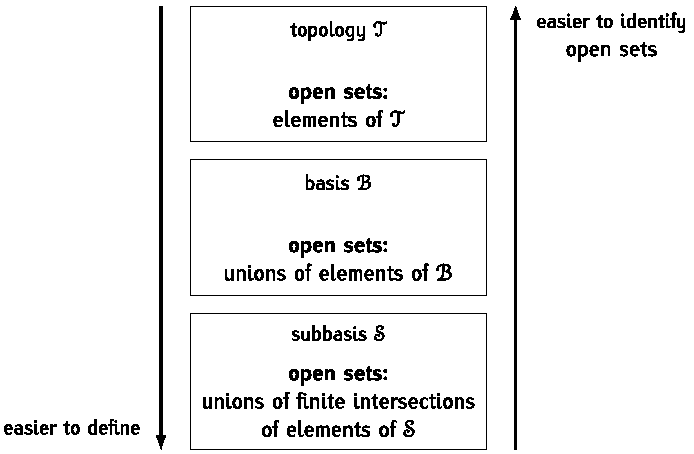
\includegraphics[width=0.7\textwidth]{Figures/topoly_(sub)basis.pdf}
		\caption{Figure taken from \cite{src:topology_sub_basis}.}
		\label{fig:topology_sub_basis}
	\end{figure}
\end{remark}

\begin{remark}\label{remark:topology_generated_by_topology}
	Let $(X, \tau)$ be a topological space, and since $\tau$ is a basis for itself, the topology generated by $\tau$, denoted by $\mathscr T(\tau)$, is $\tau$, since by Theorem \ref{thrm:gen_top_by_coll_subsets},
	$$\mathscr T(\tau) = \left\{ \bigcup_{C\in\mathscr C}C \mid \mathscr C \subset \tau \right\} = \tau,$$ since for any $\mathscr C\subset\tau$, the union of open sets is an open set again, and for every open set $U\in\tau$, consider $\mathscr C = \{U\}\subset \tau$, and thus $\bigcup_{C\in\mathscr C}C = U$.
\end{remark}

\begin{theorem}
	Let $(X, \tau_X)$ and $(Y, \tau_Y)$ be topological spaces. Then the following properties of a function $f: X\to Y$ are equivalent \cite{topology-singh}:
	\begin{enumerate}[label=(\alph*)]
		\item $f$ is an open map.
		\item For every $x\in X$ and each neighborhood $U$ of $x\in X$, there is a neighborhood $W$ of $f(x)$ in $Y$ with $W\subset f(U)$.
		\item For every $x\in X$ and each basic neighborhood $B$ of $x\in X$, $f(B)$ is a neighborhood of $f(x)$ in $Y$.
		\item The image of each member of a basis for $X$ is open in $Y$.
	\end{enumerate}
\end{theorem}

\begin{proof}
	\enquote{(a) $\Rightarrow$ (b)} Let $U$ be a neighborhood of an $x\in X$, then there exists an open set $O\in \tau_X$ s.t. $x\in O\subset U$. Define $W := f(O)$, then $W\in \tau_Y$, since $f$ is an open map, and $W\subset f(U)$, since $O\subset U$.
	
	\enquote{(b) $\Rightarrow$ (c)} Let $B$ be a neighborhood of $x\in X$, then there is a neighborhood $W$ of $f(x)$ in $Y$ s.t. $f(x)\in V\subset W\subset f(B)$, where $V\in \tau_Y$, and thus $f(B)$ is a neighborhood of $f(x)$ in $Y$.
	
	\enquote{(c) $\Rightarrow$ (d)} Use Theorem \ref{thrm:open_via_nbd}. 
	
	\enquote{(d) $\Rightarrow$ (a)} Let $\mathscr B$ be a basis for the topology on $X$, and $f(B)\in \tau_Y$ for all $B\in\mathscr B$. An open $U\subset X$ can be written as the union of a collection $\{B_i\}_{i\in I}\subset \mathscr B$, where $I$ is an index set, and thus:
	$$f(U) = f\left(\bigcup_{i\in I}B_i\right) = \bigcup_{i\in I}f(B_i) \in \tau_Y.$$
\end{proof} 

\begin{exmp}[Metric topology]\label{exmp:metric_topology}
	In a metric space $X$, the collection of all open balls 
	\begin{align}\label{eq:bases_open_ball_metric_spaces}
		\mathscr B := \{ B_{r}(x) \mid x\in X, r > 0 \}
	\end{align} 
	generates the topology $$\tau(\mathscr B) = \{U\subset X\mid \forall x\in U\ \exists B_{r}(x)\in\mathscr B: x\in B_{r}(x)\subset U\},$$
	called the \textit{metric topology}, cf. Eq. \eqref{eq:gen_top_by_coll_subsets} and Theorem \ref{thrm:gen_top_by_coll_subsets}, and $\mathscr B$ is a basis for $\tau(\mathscr B)$. This holds because for any fixed $r > 0$, $X = \bigcup_{x\in X}B_{r}(x)$, and for any point in the the intersection of two open balls, there is an open ball containing that point, and the open ball is contained in the intersection, cf. Theorem \ref{thrm:intersection_open_balls}.
\end{exmp}

\begin{remark}
	Note that it is important to consider the collection of \textit{all} open balls in Example \ref{exmp:metric_topology}. For if we considered the collection of all open balls with \textit{fixed} radius $r > 0$, it is not guaranteed that for all $B_{r}(x)$ and $B_{r}(x')$ and each point $y\in B_{r}(x)\cap B_{r}(x')$, we can find a $B_{r}(z)$ with $z\in X$ s.t. $y\in B_{r}(z)\subset B_{r}(x)\cap B_{r}(x')$, also cf. Fig. \ref{fig:open_balls_intersection}.
\end{remark}

\begin{exmp}\label{exmp:basis_discrete_metric}
	Let $(X, d)$ be a metric space, where $d$ is the discrete metric from Remark \ref{remark:discrete-metric}. Then the collection $\mathscr B := \{\varphi\in X\}\cup \{X\}$, which is the colection of all open balls, cf. Example \ref{exmp:open-balls-discrete-metric}, generates a topology $\tau(\mathscr B)$ on $X$ by Example \ref{exmp:metric_topology}, for which $\mathscr B$ is a basis. The generated topology on $X$ is the discrete topology from Example \ref{exmp:discrete_topology}. Note that $\mathscr B' := \{\varphi\in X\}$ generates the same topology on $X$.
\end{exmp}

\begin{defn}[Metrizable topological space \cite{topology-singh}]
	Let $(X, \tau)$ be a topological space, then it is called \textit{metrizable} if there is a metric $d$ on $X$, whose collection of all open balls generates the topology $\tau$.
\end{defn}

\begin{defn}[Standard topology of $\mathbb R$]\label{defn:standard_topology}
	Let $X = \mathbb R$, and $d$ the usual metric on $X$. Then for $\varphi\in X$ and $r > 0$, the open ball is $$B_{r}(\varphi) = \{ \psi\in X\mid \abs{\varphi - \psi} < r \} = (\varphi - r, \varphi + r),$$ and the collection of all such open balls is $$\mathscr B = \{(\varphi - r, \varphi + r) \mid \varphi\in X, r > 0\} = \left\{(a, b) \mid a, b\in X, a < b\right\},$$
	and the topology generated by this basis is called the \textit{standard topology} of $\mathbb R$.
\end{defn}

\begin{defn}[Lower limit topology of $\mathbb R$]
	Let $X = \mathbb R$, and $\mathscr B$ the collection of all right half-open intervals, i.e. $\mathscr B= \left\{ [a, b) \mid a, b\in\mathbb R, a < b \right\}$. Clearly, there is a collection of right half-open intervals s.t. $\mathbb R$ equals to its union, and the intersection of two right half-open intervals is either empty or itself a right half-open interval. Thus, for all $x$ in the intersection there is a right half-open interval that contains $x$ and is contained in the intersection. Thus, by Theorem \ref{thrm:gen_top_by_coll_subsets}, $\mathscr B$ generates a topology, which is called the \textit{lower limit topology} of $\mathbb R$.
\end{defn}

\begin{defn}[Upper limit topology of $\mathbb R$]
	Let $X = \mathbb R$, and $\mathscr B$ the collection of all left half-open intervals, i.e. $\mathscr B= \left\{ (a, b] \mid a, b\in\mathbb R, a < b \right\}$. Clearly, there is a collection of left half-open intervals s.t. $\mathbb R$ equals to its union, and the intersection of two left half-open intervals is either empty or itself a left half-open interval. Thus, for all $x$ in the intersection there is a left half-open interval that contains $x$ and is contained in the intersection. Thus, by Theorem \ref{thrm:gen_top_by_coll_subsets}, $\mathscr B$ generates a topology, which is called the \textit{upper limit topology} of $\mathbb R$.
\end{defn}

\begin{remark}
	Let $X = \mathbb R$, and $\mathscr B$ the collection of all closed intervals, i.e. $\mathscr B = \left\{ [a, b]\mid a, b\in\mathbb R, a \leq b \right\}$. Note that there is a collection of closed intervals s.t. $\mathbb R$ is its union, and the intersection of two closed intervals is either empty or closed. Thus, for all $x$ in the intersection, there is a closed interval that contains $x$ and that is contained in the intersection. Thus, by Theorem \ref{thrm:gen_top_by_coll_subsets}, $\mathscr B$ generates a topology, which is the discrete topology on $\mathbb R$, i.e. $\tau(\mathscr B) = \mathscr P(\mathbb R)$, since for any $x\in \mathbb R$, we have $x\in [x, x]\in \mathscr B$.
\end{remark}

\begin{remark}
	The lower and upper limit topologies of $\mathbb R$ are not metrizable \cite{790629}.
\end{remark}

\begin{exmp}
	The order topology on $\mathbb R$ (with the usual order relation) conincides with the standard topology of $\mathbb R$, since all open rays $(-\infty, a)$ and $(a, \infty)$ can be written as a union of open intervals. Conversely, every open interval, which is an open set in the standard topology, is contained in the order topology.
\end{exmp}

\begin{defn}\label{defn:euclidean_topology}
	The \textit{Euclidean topology} of $\mathbb R^n$ is generated by the basis of open balls, where the metric is the Euclidean metric.
\end{defn}	

\begin{theorem}\label{thrm:comp_topologies_bases}
	Let $\tau(\mathscr B)$ and $\tau(\mathscr B')$ be topologies on $X$ generated by the bases $\mathscr B$ and $\mathscr B'$ respectively, cf. Theorem \ref{thrm:gen_top_by_coll_subsets}. Then we have:
	$$\tau(\mathscr B)\subset \tau(\mathscr B') \ (\tau(\mathscr B)\ \text{is coarser than}\ \tau(\mathscr B')) \Leftrightarrow \forall B\in\mathscr B\ \forall x\in B\ \exists B'\in\mathscr B': x\in B'\subset B.$$
\end{theorem}

\begin{proof}
	\enquote{$\Longrightarrow$} Let $\tau(\mathscr B)\subset \tau(\mathscr B')$, then for all $B\in\mathscr B$, we have $B\in\tau(\mathscr B)$, and thus $B\in \tau(\mathscr B')$, i.e. by construction, for all $x\in B$ there exists a $B_x'\in\mathscr B'$ s.t. $x\in B_x'\subset B$.
	
	\enquote{$\Longleftarrow$} Let $U\in\tau(\mathscr B)$, i.e. for all $x\in U$ there exists a $B_x\in \mathscr B$ s.t. $x\in B_x\subset U$. By assumption, to this $B_x\in\mathscr B$, there exists a $B_x'\in\mathscr B'$ s.t. $x\in B_{x'} \subset B_x\subset U$, which shows that $U\in\tau(\mathscr B')$.
\end{proof} 

\begin{corollary}\label{corollary:equality_of_topologies}
	Let $\tau(\mathscr B)$ and $\tau(\mathscr B')$ be topologies on $X$ generated by the bases $\mathscr B$ and $\mathscr B'$ respectively, then $\tau(\mathscr B) = \tau(\mathscr B')$ iff for each $B\in \mathscr B$ and $x\in B$, there exists a $B'\in\mathscr B'$ s.t. $x\in B'\subset B$, and for each $B'\in \mathscr B'$ and $x\in B'$ there exists a $B\in\mathscr B$ s.t. $x\in B\subset B'$.
\end{corollary}

\begin{remark}
	Let $X = \mathbb R$, and denote by $\tau$ its standard topology, by $\tau_l$ the lower limit topology, and by $\tau_u$ the upper limit topology. Then $\tau\subset \tau_l$ and $\tau\subset \tau_u$, i.e. the standard topology is coarser than the lower and upper limit topologies, since for all open intervals in $\tau$ of the form $(a, b)$ with $a, b\in\mathbb R$ and $a < b$, and all points $x\in (a, b)$, the right half-open interval $[x, b)$ contains $x$ and is a subset of $(a, b)$, and the left half-open interval $(a, x]$ contains $x$ and is a subset of $(a, b)$. Thus, $\tau$ is coarser than $\tau_l$ and $\tau_u$, cf. Theorem \ref{thrm:comp_topologies_bases}. However, note that the standard topology is not equal to either the lower or upper limit topology, since there is no open interval that would be contained in intervals of the form $[a, b)$ or $(a, b]$ and contain each point of the intervals.
\end{remark}

\begin{remark}
	Let $\tau(\mathscr B)$ be the topology on $X$ generated by the basis $\mathscr B$, then Corollary \ref{corollary:equality_of_topologies} implies that there might be another, distinct basis $\mathscr B'$ s.t. $\tau(\mathscr B) = \tau(\mathscr B')$.
\end{remark}

\begin{exmp}
	Let $X = \{ a, b, c \}$, then $\mathscr B = \left\{ \{a, b\}, \{b, c \}, \{c, a\}, \{a\}, \{b\}, \{c\}\right\}$ and $\mathscr B' = \left\{ \{a\}, \{b\}, \{c\} \right\}$ are collection of subsets of $X$ s.t. the requirements of Theorem \ref{thrm:gen_top_by_coll_subsets} are fulfilled \cite{1333309}, and we have $\tau(\mathscr B) = \left\{ \emptyset, \{a\}, \{b\}, \{c\}, \{a, b\}, \{b, c\}, \{c, a\}, X \right\} = \tau(\mathscr B')$.
\end{exmp}

\begin{exmp}
	Let $X=\mathbb R$, and $\mathscr B$ the collection of all open intervals, then $\tau(\mathscr B)$ is the standard topology, cf. Example \ref{defn:standard_topology}. Now fix $c, d\in\mathbb R$, and consider $$\mathscr B' := \{(a, b) \mid a,b\in\mathbb R, a < b, a\ne c \wedge b\ne d\},$$ i.e. the collection of all open intervals, where one specific interval was removed. Since $\mathscr B'$ fulfills the requirements of Theorem \ref{thrm:gen_top_by_coll_subsets}, it generates the topology $\tau(\mathscr B')$. Clearly, by Corollary \ref{corollary:equality_of_topologies}, $\tau(\mathscr B) = \tau(\mathscr B')$, and since $c, d$ were arbitrary, it means that there infinitely many bases generating the standard topology of $\mathbb R$.
\end{exmp}

\begin{remark}
	Let $X=\mathbb R$, and consider the collection of all open intervals with rational endpoints, i.e. 
	$$\mathscr B = \{(a, b)\mid a, b\in\mathbb Q, a < b\}.$$ Clearly, $\mathbb R$ can be written as the union of all such intervals, and the intersection of two open intervals is either empty or an open interval again. Thus, $\mathscr B$ fulfills the requirements of Theorem \ref{thrm:gen_top_by_coll_subsets}, and the generated topology is the standard topology of $\mathbb R$. To see this, consider an open interval of the form $(a, b)$ with $a, b\in\mathbb R$ and $a\ne b$. Then for all $x\in (a, b)$, by the Archimedean property of $\mathbb R$, cf. Theorem \ref{thrm:between_two_reals_rational}, we know that there is $p\in\mathbb Q$ s.t. $a < p < x$ and a $q\in\mathbb Q$ s.t. $x < q < b$, thus $(p, q)$ contains $x$ and $(p, q) \subset (a, b)$. Conversely, if we choose $(p, q)\in\mathscr B$, note that $p, q\in\mathbb Q\subset \mathbb R$, and thus by Corollary \ref{corollary:equality_of_topologies}, $\tau(\mathscr B)$ also generates the standard topology of $\mathbb R$.
\end{remark}

\begin{defn}[Topological equivalence of metrics \cite{topology-singh}]\label{defn:topological_equivalence_metrics}
	Let $(X, d)$ and $(X, d')$ be metric spaces. We denote by $\mathscr B$ the collection of all $d$-open balls, generating the metric topology $\tau(\mathscr B)$, cf. Example \ref{exmp:metric_topology}, and by $\tau(\mathscr B')$ the collection of all $d'$-open balls generating the metric topology $\tau(\mathscr B')$. If $\tau(\mathscr B) = \tau(\mathscr B')$, we say that $d$ and $d'$ are \textit{(topologically) equivalent}.
\end{defn}

\begin{theorem}\label{thrm:topological_equivalence}
	Two metrics $d$ and $d'$ on a set $X$ are equivalent if and only if for each $x\in X$ and for each $\epsilon > 0$, there exist real numbers $\delta_1$, $\delta_2 > 0$ (depending upon $x$ and $\epsilon$) such that $B^{d}_{\delta_1}(x) \subset B^{d'}_{\epsilon}(x)$ and $B^{d'}_{\delta_2}(x) \subset B^{d}_{\epsilon}(x)$. \cite{topology-singh}.
\end{theorem}

\begin{proof}
	Let the notation be as in Definition \ref{defn:topological_equivalence_metrics}.
	\\
	
	\enquote{$\Longrightarrow$} For each $x\in X$ and for each $\epsilon > 0$, the open ball $B^{d}_{\epsilon}(x)\in\mathscr B$ in the metric space $(X, d)$ is open in the topology $\tau(\mathscr B)$, and the open ball $B^{d'}_{\epsilon}(x)\in\mathscr B'$ in the metric space $(X, d')$ is open in the topology $\tau(\mathscr B')$. Hence, by Corollary \ref{corollary:equality_of_topologies}, there exist $\delta_1$, $\delta_2$ such that $B^{d'}_{\delta_1}(x) \subset B^{d}_{\epsilon}(x)$ and $B^{d}_{\delta_2}(x) \subset B^{d'}_{\epsilon}(x)$.
	
	\enquote{$\Longleftarrow$} Suppose that $B^{d'}_{\delta_1}(x) \subset B^{d}_{\epsilon}(x)$ and $B^{d}_{\delta_2}(x) \subset B^{d'}_{\epsilon}(x)$ hold for each $x\in X$ and $\epsilon > 0$. Given an open set $U\subset X$ in the topology $\tau(\mathscr B)$ and a point $x\in U$, there exists an open ball $B^{d}_{r}(x) \subset U$ with $r > 0$. By assumption, there exists an open ball $B^{d'}_{\delta_1}(x) \subset B^{d}_{r}(x) \subset U$, proving that $U$ is an open set in the topology $\tau(\mathscr B')$. Similarly, one can show that every open set in the topology $\tau(\mathscr B')$ is also open in $\tau(\mathscr B)$. Hence, by Corollary \ref{corollary:equality_of_topologies}, $\tau(\mathscr B) = \tau(\mathscr B')$.
\end{proof}

\begin{theorem}
	If two metrics $d$ and $d'$ on a set $X$ are strongly equivalent, cf. Def. \ref{defn:strong_equivalence}, then they are also (topologically) equivalent.
\end{theorem}

\begin{proof}\cite{1379634}
	By definition of strong equivalence, we know that 
	\begin{align}
		\alpha d(x, y) \leq d'(x, y) \leq \beta d(x, y) \quad\forall x, y\in X, \alpha, \beta > 0.
	\end{align}
	According to Theorem \ref{thrm:topological_equivalence}, we need to show that for all $x\in X$ and $\epsilon > 0$, there exist $\delta_1$, $\delta_2 > 0$ such that 
	\begin{align}
		\left(B_{\delta_1}^{d}(x) \subset B_{\epsilon}^{d'}(x)\right) \wedge \left(B^{d'}_{\delta_2}(x) \subset B^{d}_{\epsilon}(x)\right)
	\end{align}
	To show the first inclusion, let $\delta_1 \leq \epsilon/\beta$, then we have for all $x$, $y\in X$:
	\begin{align}
		\frac{d'(x, y)}{\beta} \leq d(x, y) < \delta_1 \leq \frac{\epsilon}{\beta} \Rightarrow d'(x, y) < \epsilon.
	\end{align}
	To show the second inclusion, let $\delta_2 \leq \epsilon\alpha$, then we have for all $x$, $y\in X$:
	\begin{align}
		\alpha d(x, y)\leq d'(x, y) < \delta_2 \leq \epsilon\alpha \Rightarrow d(x, y) < \epsilon.
	\end{align}
\end{proof}

\begin{theorem}\label{thrm:new_metric_top_equivalent}
	Let $(X, d)$ be a metric space, and consider the metric $$\rho(x, y) := \frac{d(x, y)}{1 + d(x, y)} $$ for all $x, y\in X$, cf. Theorem \ref{thrm:new_metric_out_of_given_metric}. Then $d$ and $\rho$ are topologically equivalent.
\end{theorem}

\begin{proof}
	Choose arbitrary $x\in X$ and $\epsilon > 0$. Choose $\delta_1 := \epsilon/(1 - \epsilon)$, then $B_{\delta_1}^{d}(x) \subset B_{\epsilon}^{\rho}(x)$, since for any $y\in B_{\delta_1}^{d}(x)$, we have 
	\begin{align*}
		d(x, y) < \delta_1 &= \frac{\epsilon}{1 - \epsilon} \Leftrightarrow d(x, y) - \epsilon d(x, y) < \epsilon \Leftrightarrow d(x, y) < \epsilon + \epsilon d(x, y) = \epsilon (1 + d(x, y))
		\\ \Leftrightarrow \frac{d(x, y)}{1 + d(x, y)} &= \rho(x, y) \leq \epsilon,
	\end{align*}
	i.e. $y\in B_{\epsilon}^{\rho}(x)$. Conversely, choose $\delta_2 := \epsilon$, then $B_{\delta_2}^{\rho}(x) \subset B_{\epsilon}^{d}(x)$, since for any $y\in B_{\delta_2}^{\rho}(x)$, $\rho(x, y) \leq d(x, y)$.
	
	Thus, by Theorem \ref{thrm:topological_equivalence}, $d$ and $\rho$ are topologically equivalent.
\end{proof}

\begin{remark}
	There exist metrics $d$ and $d'$ on a set $X$ that are (topologically) equivalent, but not strongly equivalent. \cite{5065146}
\end{remark}

\begin{exmp}
	Let $X := (0, 1]$, and for any $x$, $y\in X$, define $d(x, y) := \abs{x - y}$ and \newline $d'(x, y) := \abs{x^{-1} - y^{-1}}$. Clearly, $d$ and $d'$ define metrics on $X$, and they are not strongly equivalent, since there is no $\beta > 0$ s.t. $d'(x, y) \leq d(x, y)$ for all $x$, $y\in X$. 
	
	However, $d$ and $d'$ are (topologically) equivalent. To see this, remember that acc. to \mbox{Theorem \ref{thrm:topological_equivalence}}, we need to prove that for any $x\in X$ and for any $\epsilon > 0$, there exist $\delta_{1}(x, \epsilon)$ and $\delta_2(x, \epsilon)$ s.t. $B_{\delta_1}^{d}(x) \subset B_{\epsilon}^{d'}(x)$ and $B_{\delta_2}^{d'}(x) \subset B_{\epsilon}^{d}(x)$. 
	
	To show the first inclusion, choose any
	\begin{align}\label{eq:top-eq-not-imply-strong-eq-delta_1}
		\delta_{1} < \frac{\epsilon x^2}{\epsilon x + 1}.
	\end{align}
	Now we have 
	\begin{align}\label{eq:top-eq-not-imply-strong-eq-delta_1-2}
		y \in B_{\delta_1}^{d}(x) \Rightarrow \abs{y - x} < \delta_1 \Rightarrow \frac{1}{xy}\abs{x - y} = \abs{\frac{1}{x} - \frac{1}{y}} < \frac{\delta_1}{xy}
	\end{align}
	Since $z \leq \abs{z}$ for any $z\in\mathbb R$, 
	\begin{align}\label{eq:top-eq-not-imply-strong-eq-delta_1-3}
		y \in B_{\delta_1}^{d}(x) \Rightarrow x - y \leq \abs{x-y} < \delta_1 \Rightarrow x - \delta_1 < y\Rightarrow \frac{1}{y} < \frac{1}{x - \delta_1},
	\end{align}
	and hence 
	\begin{align}
		y \in B_{\delta_1}^{d}(x) \overset{\tiny \eqref{eq:top-eq-not-imply-strong-eq-delta_1-2}}{\Rightarrow} \abs{\frac{1}{x} - \frac{1}{y}} &< \frac{\delta_1}{xy} \overset{\tiny \eqref{eq:top-eq-not-imply-strong-eq-delta_1-3}}{<} \frac{\delta_1}{x(x - \delta_1)} = \frac{\delta_1}{x^2 - x\delta_1} \overset{\tiny \eqref{eq:top-eq-not-imply-strong-eq-delta_1}}{<} \frac{\epsilon x^2}{\left(\epsilon x + 1\right)\left(x^2 - \frac{\epsilon x^3}{\epsilon x + 1}\right)} 
		\\ &= \frac{\epsilon x^2}{\epsilon x^3 - \frac{\epsilon^2 x^4}{\epsilon x + 1} + x^2 - \frac{\epsilon x^3}{\epsilon x + 1}} = \frac{\epsilon x^2}{\frac{\epsilon^2 x^4 + \epsilon x^3}{\epsilon x + 1} - \frac{\epsilon^2 x^4}{\epsilon x + 1} + x^2 - \frac{\epsilon x^3}{\epsilon x + 1}} = \epsilon.
	\end{align}
	
	To show the second inclusion, i.e. $B_{\delta_2}^{d'}(x) \subset B_{\epsilon}^{d}(x)$, choose $\delta_2 := \epsilon$, then we have:
	\begin{align}
		y \in B_{\delta_2}^{d'}(x) \Rightarrow \abs{\frac{1}{x} - \frac{1}{y}} < \delta_2 \Rightarrow xy\abs{\frac{1}{x} - \frac{1}{y}} = \abs{y - x} < \delta_2 xy \overset{x, y\in X = (0, 1]}{\leq} \delta_2 = \epsilon.
	\end{align}
\end{exmp}

\begin{theorem}
	Two metrics $d$ and $d'$ on a set $X$ are (topologically) equivalent iff each convergent sequence in $X$ wrt $d$ is also convergent in $X$ wrt $d'$. In that case, their limits coincide.
\end{theorem}

\begin{proof}
	\enquote{$\Longrightarrow$} Let $d$ and $d'$ be equivalent metrics on $X$, and let $(\varphi_n)_{n\in\mathbb N}$ be a sequence in $X$, which converges to $\varphi\in X$ wrt $d$, i.e.
	\begin{align}
		d(\varphi, \varphi_n) \overset{n\to\infty}{\longrightarrow} 0.
	\end{align}
	According to Theorem \ref{thrm:topological_equivalence}, for any $\epsilon > 0$, there is a $\delta > 0$ s.t. $B_{\delta}^{d}(\varphi) \subset B_{\epsilon}^{d'}(\varphi)$. To this $\delta$, there exists an $N\in\mathbb N$ s.t. $d(\varphi, \varphi_n) < \delta$ for all $n\geq N$, cf. Def. \ref{defn:convergence_sequence}. Hence:
	\begin{align}
		\varphi_n\in B^{d}_{\delta}(\varphi) \subset B^{d'}_{\epsilon}(\varphi), \quad \forall n\geq N
	\end{align}
	i.e. $d'(\varphi, \varphi_n) < \epsilon$ for any $\epsilon > 0$.
	
	\enquote{$\Longleftarrow$} Let $U\subset X$ be $d$-open in $X$, i.e. open wrt $d$. Then $X\backslash U$ is $d$-closed in $X$. Let $\varphi\in X$ be a $d'$-accumulation point of $X\backslash U$, i.e. there exists a sequence $(\varphi_n)_{n\in\mathbb N}$ in $X\backslash U$ s.t. $\varphi_n \overset{d'}{\longrightarrow} \varphi$ for $n\to\infty$. By assumption, $(\varphi_n)_{n\in\mathbb N}$ converges to a $\psi\in X$ wrt $d$. Since $X\backslash U$ is closed, by Theorem \ref{thm:closed_set_acc_point}, $\psi\in X\backslash U$ holds. 
	
	Let us now show that $\varphi = \psi$. For this, consider the extended sequence 
	\begin{align}
		\left(\varphi_1, \varphi, \varphi_2, \varphi, \varphi_3, \varphi, \dots\right).
	\end{align}
	The extended sequence converges to $\varphi$ wrt $d'$, and hence it also converges wrt $d$. The subsequence $(\varphi_n)_{n\in\mathbb N}$ of the extended sequence converges to $\psi$ wrt $d$. Hence, $\varphi = \psi$, and the $d'$-accumulation point $\varphi=\psi$ of $X\backslash U$ lies in $X\backslash U$, i.e. $X\backslash U$ is also $d'$-closed (by Theorem \ref{thm:closed_set_acc_point}). This in turn implies that $U$ is $d'$-open.
	
	We have shown that $d$ and $d'$ induce the same topology on $X$, and are hence equivalent.
\end{proof}

\begin{theorem}\label{thrm:equivalent_metric_finite_diameter}
	Let $(X, \tau)$ be a metrizable topological space, and $d$ a metric on $X$ inducing $\tau$. Then for each $\lambda > 0$ there exists a metric $d_{\lambda}$ on $X$ s.t. $d_{\lambda}$ is (topologically) equivalent to $d$ and $\text{diam}(X) \leq \lambda$ wrt $d_{\lambda}$ \cite{topology-singh}.
\end{theorem}

\begin{proof}
	For all $x, y\in X$, define $d_{\lambda}(x, y) := \min\{\lambda, d(x, y)\}$. Clearly, $d_{\lambda}$ is positive, and $$d_{\lambda}(x, y) = \min\{\lambda, d(x, y)\} = 0\Leftrightarrow d(x, y) = 0\Leftrightarrow x = y,$$ i.e. $d_{\lambda}$ is also definite.
	Clearly, $d_{\lambda}$ is symmetric, to prove the triangle inequality, let $z\in X$, and note that
	\begin{align*}
		d_{\lambda}(x, z) &= \min\{\lambda, d(x, z)\} \leq \min\{ \lambda, d(x, y) + d(y, z) \} \\ &\leq \min\{\lambda, d(x, y)\} + \min\{\lambda, d(y, z)\} = d_{\lambda}(x, y) + d_{\lambda}(y, z).
	\end{align*}
	Thus, $d_{\lambda}$ is a metric on $X$, and clearly $\text{diam}(X)\leq\lambda$ wrt $d_{\lambda}$. 
	
	For all $x\in X$ and $\epsilon > 0$, we have 
	$$B^{d}_{\epsilon}(x)  = \left\{y\in X\mid d(x, y) < \epsilon\right\} \subset \{y\in X\mid \min\{\lambda, d(x, y)\} < \epsilon\} = B_{\epsilon}^{d_{\lambda}}(x)$$
	and for $\delta := \min\{\lambda, \epsilon\}$, we have
	$$B^{d_{\lambda}}_{\delta}(x) = \left\{y\in X\mid \min\{\lambda, d(x, y)\} < \min\{\lambda, \epsilon\}\right\} \subset B^{d}_{\epsilon}(x),$$
	since if $d_{\lambda}(x, y) = d(x, y)$, then $d(x, y) < \epsilon$, otherwise $d_{\lambda}(x, y) = \lambda$. In that case, if $\epsilon\leq \lambda$, we have $\min\{\lambda, \epsilon\} = \epsilon$, and thus there is no $y\in X$ fulfilling $\lambda < \epsilon$, i.e. $B_{\delta}^{d_{\lambda}}(x) = \{x\}\subset B_{\epsilon}^{d}(x)$. Otherwise, $\lambda < \epsilon$, but there is no $y\in X$ fulfilling $\lambda < \lambda$, i.e. $B_{\delta}^{d_{\lambda}}(x) = \{x\}\subset B_{\epsilon}^{d}(x)$. Thus, by Theorem \ref{thrm:topological_equivalence}, $d_{\lambda}$ is topologically equivalent to $d$.
\end{proof}

Let us now look at what topological structure we can endow $X\times Y := \{ (x, y) \mid x\in X, y\in Y \}$ with if $(X, \tau_X)$ and $(Y, \tau_Y)$ are topological spaces.

\begin{remark}
	The naive way would be to define the collection of open sets as 
	\begin{align}\label{eq:basis_product_topology}
		\mathscr B := \{ U\times V \mid U\in\tau_X, V\in\tau_Y \}\subset \mathcal P(X\times Y).
	\end{align}
	While $\emptyset\in\mathscr B$ (since $\emptyset\in \tau_X$, $Y\in \tau_Y$, and $\emptyset\times Y = \emptyset$), $X\times Y \in \mathscr B$, and if $U_1\times V_1\in\mathscr B$ and $U_2\times V_2\in\mathscr B$, then $(U_1\times V_1) \cap (U_2\times V_2)\in\mathscr B$, i.e. the intersection of two members of $\mathscr B$ is also in $\mathscr B$ again\footnote{This holds because 
		\begin{align*}
			(U_1 \times V_1) \cap (U_2\times V_2) &= \{(u, v) \mid (u, v)\in U_1\times V_1 \wedge (u, v)\in U_2\times V_2 \} \\ &= \{(u, v) \mid u\in U_1\wedge v\in V_1\wedge u\in U_2\wedge v\in V_2\}
			\\ &= \{(u, v)\mid u\in U_1\cap U_2 \wedge v\in V_1\cap V_2\}
			\\ &= (U_1\cap U_2) \times (V_1\cap V_2),
		\end{align*}
		and we have $U_1, U_2\in\tau_X$ and $V_1, V_2\in\tau_Y$, i.e. $U_1\cap U_2\in\tau_X$ and $V_1\cap V_2\in \tau_Y$.
	}. However, note that the union of two members of $\mathscr B$ is not necessarily in $\mathscr B$ again. For example, consider these two rectangles, then their union is clearly not a rectangle again:
	\begin{figure}[h!]
		\centering 
		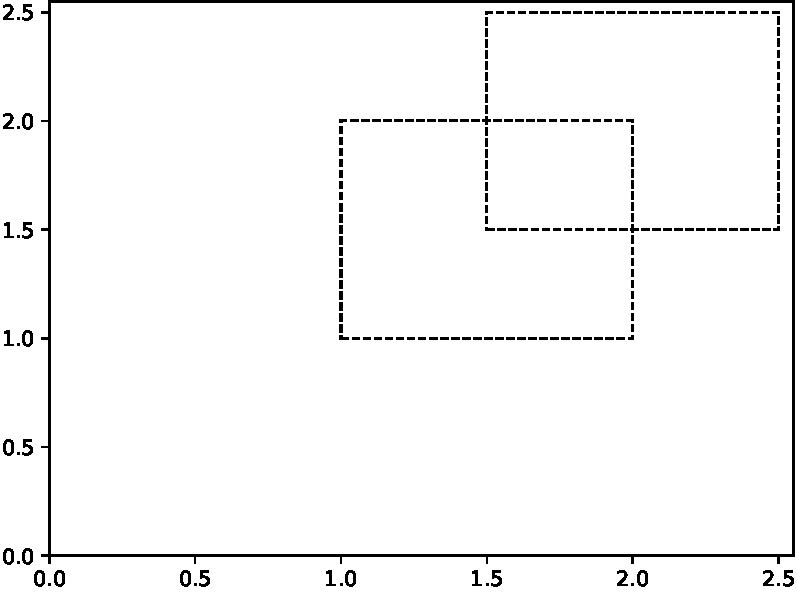
\includegraphics[width=0.6\textwidth]{scripts/rectangles.pdf}
	\end{figure}
	
	Mathematically, we can describe these two rectangles as $(1, 2) \times (1, 2)$ and $(1.5, 2.5) \times (1.5, 2.5)$, and we consider $X = Y = \mathbb R$ with the standard topology.
\end{remark}

\begin{defn}[Product topology \cite{topology-singh}]\label{defn:product_topology}
	Let $\mathscr B$ be defined as in Eq. \ref{eq:basis_product_topology}, then $\mathscr B$ fulfills the requirements of Theorem \ref{thrm:gen_top_by_coll_subsets}, and thus $\mathscr B$ generates a topology $\tau(\mathscr B)$ on $X\times Y$, called the \textit{product topology}. When $X \times Y$ is equipped with the product topology, it is also called the \textit{product space}; $X$ and $Y$ are called the \textit{coordinate spaces}. The maps
	\begin{equation}
		\begin{aligned}
			p_X: X\times Y\to X, (x, y) &\mapsto x, \label{eq:projections_coord_spaces} 
			\\ p_Y: X\times Y\to Y, (x, y)&\mapsto y
		\end{aligned}
	\end{equation}
	are projections of the product space $X\times Y$ onto the coordinates spaces.
\end{defn}

\begin{theorem}\label{thrm:prod_top_continuous_projs}
	Let $(X, \tau_X)$ and $(Y, \tau_Y)$ be topological spaces. The projections $p_X$ and $p_Y$ from the product space onto the coordinates spaces, cf. Eq. \eqref{eq:projections_coord_spaces}, are continuous, the product topology is the smallest topology for which this is true, and $p_X$ and $p_Y$ are open maps.
\end{theorem}

\begin{proof}
	Let $U\in \tau_X$, then $$p_X^{-1}(U) = \left\{(x, y)\in X\times Y \mid p_X((x, y))\in U\right\} = \left\{(x, y)\in X\times Y \mid x\in U\right\} = U\times Y,$$ and thus $p_X$ is continuous in the product topology on $X\times Y$, cf. Definition \ref{defn:continuity_topological_spaces}. Similarly, we can show the continuity of $p_Y$.
	
	Now suppose there is a topology $\mathscr T$ on $X\times Y$ s.t. both $p_X$ and $p_Y$ are continuous. Let $U\in \tau_X$ and $V\in\tau_Y$, then $p_X^{-1}(U) = U\times Y\in \mathscr T$, $p_Y^{-1}(V) = X\times V\in \mathscr T$, and thus
	\begin{align}\label{eq:intersection_of_preimage_of_projs}
		p_X^{-1}(U) \cap p_Y^{-1}(V) = (U\times Y)\cap (X\times V) = (U\cap X) \times (Y\cap V) = U\times V,
	\end{align}
	i.e. all basis members of the product topology on $X\times Y$ are contained in $\mathscr T$ (note that $\mathscr T$ is a basis for itself, generating $\mathscr T$, cf. Remark \ref{remark:topology_generated_by_topology}), and thus by Theorem \ref{thrm:comp_topologies_bases}, $\mathscr T$ is finer than the product topology on $X\times Y$, i.e. the product topology is the smallest topology on which $p_X$ and $p_Y$ are continuous.
	
	Finally, note that $p_X$ and $p_Y$ are open maps. To see this, note that if $U\in\tau_X$ and $V\in\tau_Y$, then $U\times V$ is open in the product topology, and $p_X(U\times V) = U\in\tau_X$ and $p_Y(U\times V) = V\in\tau_Y$.
\end{proof}

\begin{remark}\label{remark:subbasis_prod_topology}
	Define $\mathscr S := \left\{ p_X^{-1}(U) \mid U\in\tau_X \right\} \cup \left\{ p_Y^{-1}(V) \mid V\in\tau_Y \right\}$, then $\mathscr S$ is a subbasis for the product topology on $X\times Y$, since $p_X^{-1}(U) \cap p_Y^{-1}(V) = U\times V\in \mathscr B$, cf. Eq. \eqref{eq:intersection_of_preimage_of_projs} and \eqref{eq:basis_product_topology}.
\end{remark}

If bases of the coordinate spaces are known, then we can construct a smaller basis for the product topology than in Eq. \eqref{eq:basis_product_topology}.

\begin{theorem}\label{thrm:basis_product_topology_coarser}
	Let $\mathscr C$ be a basis for $\tau_X$, and $\mathscr D$ be a basis for $\tau_Y$, then
	$$\mathscr B' := \left\{C\times D \mid C\in \mathscr C, D\in \mathscr D\right\}$$
	is a basis for the product topology on $X\times Y$.
\end{theorem}

\begin{proof}
	By Definition \ref{defn:product_topology}, $\mathscr B = \{ U\times V \mid U\in\tau_X, V\in\tau_Y \}$ is a basis for the product topology on $X\times Y$. Let $U\times V\in \mathscr B$, i.e. $U\in\tau_X$ and $V\in\tau_Y$. Then by Theorem \ref{thrm:collection_of_subsets_basis}, for all $x\in U$ there is a $C_x\in \mathscr C$ s.t. $x\in C_x\subset U$, and for all $y\in V$ there is a $D_y\in\mathscr D$ s.t. $y\in D_y\subset V$. Thus, for all $U\times V\in \mathscr B$ and all $(x, y)\in U\times V$, there is $C_x\times D_y\in \mathscr B'$ s.t. $(x, y)\in C_x\times D_y\subset U\times V$.
	
	Conversely, if $C\times D\in \mathscr B'$, i.e. $C\in\mathscr C$ and $D\in\mathscr D$, then $C\times D\in\mathscr B$, and thus by Corollary \ref{corollary:equality_of_topologies}, $\mathscr B'$ generates the product topology on $X\times Y$.
\end{proof}

\begin{remark}
	Let $(X, \tau_X)$ and $(Y, \tau_Y)$ be topological spaces, $A\subset X$ and $B\subset Y$. There are two ways in which we can define a topology on $A\times B$. First, notice that $A\times B\subset X\times Y$, and thus we can endow $A\times B$ with the subspace topology, cf. Theorem \ref{thrm:subspace_topology}. According to Theorem \ref{thrm:subspace_basis}, sets of the form $(A\times B) \cap (U\times V)$, where $U\in\tau_X$ and $V\in\tau_Y$, are members of the basis for this topology.
	
	Since $A\subset X$, $A$ is endowed with the subspace topology from $X$, similarly for $B\subset Y$, and thus $A\times B$ is the product topology of the subspace topologies on $A$ and $B$, where the basis members are of form $(A\cap U)\times (B\cap V)$ for $U\in\tau_X$ and $V\in\tau_Y$. Note that $(A\cap U)\times (B\cap V) = (A\times B)\cap (U\times V)$, and thus both topologies coincide.
\end{remark}

\begin{theorem}\label{thrm:prod_top_continuity_comps_projs}
	Let $X, Y, Z$ be topological spaces. A function $f: Z\to X\times Y$ is continuous iff the compositions $p_X\circ f: Z\to X$ and $p_Y\circ f: Z\to Y$ are continuous.
\end{theorem}

\begin{proof}
	\enquote{$\Longrightarrow$} If $f$ is continuous, then $p_X\circ f$ and $p_Y\circ f$ are continuous, since they are the composition of continuous functions.
	
	\enquote{$\Longleftarrow$} Let $p_X\circ f$ and $p_Y\circ f$ be continuous. Let $U\subset X$ and $V\subset Y$ be open, then we want to show that $f^{-1}(U\times V) = \{z\in Z\mid f(z)\in U\times V\}$ is open in $Z$. For this, note that $$\left(p_X\circ f\right)^{-1}(U) \cap \left(p_Y\circ f\right)^{-1}(V) = \{z\in Z\mid (p_X\circ f)(z) \in U\} \cap \{z\in Z\mid (p_Y\circ f)(z)\in V\}$$ and
	\begin{align*}
		z\in f^{-1}(U\times V) &\Leftrightarrow f(z)\in U\times V \Leftrightarrow (p_X\circ f)(z) \in U \wedge (p_Y\circ f)(z)\in V
		\\ &\Leftrightarrow z\in (p_X\circ f)^{-1}(U)\cap (p_Y\circ f)^{-1}(V),
	\end{align*}
	i.e. $f^{-1}(U\times V) = (p_X\circ f)^{-1}(U)\cap (p_Y\circ f)^{-1}(V)$, and since $p_X\circ f$ and $p_Y\circ f$ are continuous by assumption, $(p_X\circ f)^{-1}(U)$ and $(p_Y\circ f)^{-1}(V)$ are open in $Z$, and so is their intersection.
\end{proof}

\begin{remark}\label{remark:op_prod_top_spaces_comm_associat}
	Let $(X, \tau_X), (Y, \tau_Y)$ and $(Z, \tau_Z)$ be topological spaces. The operation of forming the product of topological spaces is commutative, in the sense that there is an obvious canonical homeomorphism $$f: X\times Y\to Y\times X, (x, y)\mapsto (y, x),$$ where $X\times Y$ is equipped with the product topology on $X\times Y$, and $Y\times X$ is equipped with the product topology on $Y\times X$. 
	
	The operation of forming the product of topological spaces is also associative, in the sense that there is an obvious canonical homeomorphism $$g: \left(X\times Y\right)\times Z\to X\times (Y\times Z), ((x, y), z)\mapsto (x, (y, z)),$$ where $(X\times Y)\times Z$ is equipped with the product topology on $(X\times Y)\times Z$, and $X\times (Y\times Z)$ is equipped with the product topology on $X\times (Y\times Z)$.
\end{remark}

\begin{proof}
	We use Theorem \ref{thrm:continuity_sub_basis} for the proof. 
	
	Clearly, $f$ and $g$ are bijective. $f$ is continuous, since a basis for the product topology on $Y\times X$ is the set $\{V\times U \mid V\in\tau_Y, U\in\tau_X \}$, and 
	\begin{align*}
		f^{-1}(V\times U) &= \{(x, y)\in X\times Y\mid f((x, y))\in V\times U\} \\ &= \{(x, y)\in X\times Y\mid (y, x)\in V\times U\} = U\times V,
	\end{align*}
	and $U\times V$ is a member of the basis for the product topology on $X\times Y$.
	
	$f^{-1}: Y\times X\to X\times Y$ is continuous, since a basis for the product topology on $X\times Y$ is $\{U\times V \mid U\in\tau_X, V\in\tau_Y \}$, and
	\begin{align*}
		\left(f^{-1}\right)^{-1}(U\times V) = f(U\times V) = \left\{f((u, v))\mid (u, v)\in U\times V\right\} = V\times U,
	\end{align*}
	and $V\times U$ is a member of the basis for the product topology on $Y\times X$.
	Thus, $f$ is a homeomorphism.
	
	$g$ is continuous, since a basis for the product topology on $X\times (Y\times Z)$ is $\{ U\times (V\times W) \mid U\in\tau_X, V\in\tau_Y, W\in\tau_Z\}$, and
	\begin{align*}
		g^{-1}(U\times (V\times W)) &= \left\{ ((x, y), z) \in (X\times Y)\times Z \mid g((x, y), z) \in U\times(V\times W) \right\}
		\\ &= \left\{ ((x, y), z) \in (X\times Y)\times Z \mid (x, (y, z)) \in U\times(V\times W) \right\}
		\\ &= (U\times V)\times W,
	\end{align*}
	and $(U\times V)\times W$ is a member of the basis for the product topology on $(X\times Y)\times Z$.
	
	Similarly, we can show that $g^{-1}$ is continuous, and thus $g$ is a homeomorphism.
\end{proof}

\begin{defn}[Product of topological spaces \cite{topology-singh}]
	Define $I := \{1, \dots, n\}$, for some $n\in\mathbb N$, and let $(X, \tau_i)$ be topological spaces for all $i\in I$, then based on Remark \ref{remark:op_prod_top_spaces_comm_associat}, we can inductively define the product of topological spaces to be 
	\begin{align}
		\prod_{i=1}^{n}X_i = X_1 \times \dots\times X_n := (X_1\times \dots\times X_{n-1})\times X_n.
	\end{align}
\end{defn}

\begin{remark}
	The results for the finite product of topological spaces follow by induction from the corresponding results for the product of two topological spaces. For example, if $(X, \tau_i)$ are topological spaces for all $i\in \{1, \dots, n\}$ for some $n\in\mathbb N$, and $\mathscr B_i$ is a basis for $\tau_i$, then Theorem \ref{thrm:basis_product_topology_coarser} implies that $\mathscr B := \left\{\prod_{i=1}^{n}U_i\mid U_i\in \mathscr B_i\right\}$ is a basis for the product topology on $\prod_{i=1}^{n}X_i$.
\end{remark}

\begin{theorem}\label{thrm:product_of_metrizable_topologies_is_metrizable}
	For all $i\in\{1, \dots, n\}$, with $n\in\mathbb N$, let $(X_i, \tau_i)$ be metrizable topological spaces. Then $\prod_{i=1}^{n}X_i$ with the product topology on it is metrizable.
\end{theorem}

\begin{proof}[Proof \cite{src:product_topology}]
	First, we construct a metric on $X := \prod_{i=1}^{n}X_i$. Since each $X_i$ is a metrizable topological space, there is a metric $d_i$ on $X_i$ inducing the topology on $X_i$. Define
	\begin{align}
		d(x, y) := \max_{1\leq i\leq n}\{d_i(x_i, y_i)\}, \quad x, y\in X.
	\end{align}
	Note that $d$ is a metric on $X$: $d$ is positive, since $d_{i}(x_i, y_i) \geq 0$, and thus $d(x, y)\geq 0$ for all $x, y\in X$. Further,
	$$d(x, y) = 0 \Leftrightarrow \forall i\in \{1, \dots, n\}: d_i(x_i, y_i) = 0 \Leftrightarrow \forall i\in \{1, \dots, n\}: x_i = y_i\Leftrightarrow x = y,$$
	i.e. $d$ is definite. Clearly, $d$ is also symmetric. Finally, for all $x, y, z\in X$, we have
	\begin{align*}
		d(x, z) = &\max_{1\leq i\leq n}\{d_i(x_i, z_i)\} \leq \max_{1\leq i\leq n}\{d_i(x_i, 
		y_i) + d_i(y_i, z_i)\} 
		\\ \overset{\tiny\eqref{thrm:max_property}}{\leq} &\max_{1\leq i\leq n}\{d_i(x_i, y_i)\} + \max_{1\leq i\leq n}\{d_i(y_i, z_i)\} = d(x, y) + d(y, z).
	\end{align*}		
	We will now prove that the topology generated (induced) by $d$ is the product topology on $X$. 
	
	For all $i\in\{1, \dots, n\}$, choose open $U_i\subset X_i$, then $U := \prod_{i=1}^{n}U_i$ is a basis member of the product topology on $X$. Since the $U_i$ are open, by Theorem \ref{thrm:collection_of_subsets_basis}, for all $u_i\in U_i$ there is an open ball $B_{\epsilon_i}(u_i)$ that is contained in $U_i$. Define $\epsilon := \min_{1\leq i\leq n}\epsilon_i > 0$, then for all $u\in U$ we have 
	\begin{align*}
		B_{\epsilon}(u) &= \left\{x\in X \mid d(x, u) < \epsilon \right\} = \left\{x\in X\mid \max_{1\leq i\leq n}\{ d_i(x_i, u_i) \} < \min_{1\leq i\leq n}\{\epsilon_i\} \right\} \\ &\overset{(\star)}{\subset} \prod_{i=1}^{n}B_{\epsilon_i}(u_i) \subset \prod_{i=1}^{n}U_i = U,
	\end{align*}
	where $(\star)$ holds, since $x\in B_{\epsilon}(u)$ implies that for all $i\in\{1, \dots, n\}$,
	$$d_i(x_i, u_i) \leq \max_{1\leq i\leq n}\{ d_i(x_i, u_i) \} < \epsilon \leq \epsilon_i,$$
	and thus for all $i$, $x_i\in B_{\epsilon_i}(u_i)$.
	
	Conversely, consider a basis member $B_{\epsilon}(x)$ of the induced topology by $d$ for some $x\in X$ and $\epsilon > 0$. Let $y\in \prod_{i=1}^{n}B_{\epsilon}(x_i)$, then for all $i$, 
	$$d_i(x_i, y_i) < \epsilon \Rightarrow \max_{1\leq i\leq n}\{d_i(x_i, y_i)\} < \epsilon \Rightarrow y\in B_{\epsilon}(x),$$
	i.e. $x\in \prod_{i=1}^{n}B_{\epsilon}(x_i)\subset B_{\epsilon}(x)$, where $\prod_{i=1}^{n}B_{\epsilon}(x_i)$ is a basis member of the product topology on $X$, since each $B_{\epsilon}(x_i)$ is a basis member of $X_i$. 
	
	By Corollary \ref{corollary:equality_of_topologies}, the induced topology by $d$ on $X$ and the product topology on $X$ coincide.
\end{proof}

\begin{remark}
	In Theorem \ref{thrm:product_of_metrizable_topologies_is_metrizable}, we constructed the metric $d(x, y) := \max_{1\leq i\leq n}\{d_i(x_i, y_i)\}$ on $X := \prod_{i=1}^{n}X_i$, where $X_i$ is a metrizable topological space, and $d_i$ a metric on $X_i$ inducing the topology on $X_i$, and showed that it induces the product topology on $X$. Note that there are other metrics on $X$ that are strongly -- and thus topologically -- equivalent to $d$ \cite{src:product_topology}, for example the $L^p$ metrics for $p\in \mathbb N\cup \{\infty\}$:
	$$d_p(x, y) := \left(\sum_{i=1}^{n}d_i(x_i, y_i)^p\right)^{1/p}, \quad x, y\in X,$$
	where $d_i$ is a metric on $X_i$, also cf. Example \ref{exmp:lp-norm-vectors}. For $p = \infty$, we obtain the maximum metric defined previously.
\end{remark}

\begin{theorem}
	Equip $\mathbb R$ with its standard topology, let $X$ be a metrizable topological space, i.e. there is a metric $d$ inducing its topology, then the metric $d: X\times X\to \mathbb R$ is continuous, when considering the product topology on $X\times X$.
\end{theorem}

\begin{proof}[Proof \cite{287313, 4228334}]
	A basis for the standard topology of $\mathbb R$ is given by open intervals $(a, b)$, where $a < b$. By Theorem \ref{thrm:continuity_sub_basis}, we need to show that the preimage of $(a, b)$ is open in the product topology; note that
	$$d^{-1}((a, b)) = \{(x, y)\in X\times X\mid d(x, y)\in (a, b)\} = \{(x, y)\in X\times X\mid a < d(x, y) < b\}.$$
	By Corollary \ref{corollary:open_set_basis_member_containment}, we only need to show that there is a basis member $B$ of the product topology of $X \times X$ s.t. for all $(x, y)\in d^{-1}((a, b))$, $(x, y)\in B\subset d^{-1}((a, b))$.
	
	Let $(x, y)\in d^{-1}((a, b))$ be arbitrary, and define $\epsilon := \min\{d(x, y) - a, b - d(x, y)\}$. Now consider $z\in B_{\epsilon}(d(x, y))$, i.e. $\abs{d(x, y) - z} < \epsilon$. Since for all $r\in\mathbb R$, $r \leq \abs{r}$ and $-r\leq \abs{r}$, we have $z\in (a, b)$, i.e. $B_{\epsilon}(d(x, y))\subset (a, b)$.
	
	Now consider $B_{\epsilon/2}(x)\times B_{\epsilon/2}(y)$, which is a basis member for the product topology on $X\times X$, and let $(x', y')\in B_{\epsilon/2}(x)\times B_{\epsilon/2}(y)$, then we have
	$$d(x', y') \leq d(x', y) + d(y, y') \leq d(x, y) + d(x', x) + d(y, y') < d(x, y) + \epsilon$$
	and 
	$$d(x, y) \leq d(x, y') + d(y', y) \leq d(x', y') + d(x', x) + d(y', y) < d(x', y') + \epsilon.$$
	Thus, $\abs{d(x, y)  - d(x', y')} < \epsilon$, which implies $d(x', y')\in B_{\epsilon}(d(x, y)) \subset (a, b)$, i.e. $(x', y')\in d^{-1}((a, b))$, which shows that $B_{\epsilon/2}(x)\times B_{\epsilon/2}(y) \subset d^{-1}(a, b)$, and we also have $(x, y)\in B_{\epsilon/2}(x)\times B_{\epsilon/2}(y)$.
\end{proof}

Let us now look at how to define a topology on the infinite Cartesian product of sets.

\begin{theorem}
	Let $A$ be an index set, and consider the collection $\{X_{\alpha}\}_{\alpha\in A}$, where $X_{\alpha}$ is a topological space for each $\alpha\in A$. Consider the set
	\begin{align}\label{basis:box_topology}
		\mathscr B := \left\{ \prod_{\alpha\in A}U_{\alpha}\mid U_{\alpha}\subset X_{\alpha}\ \text{open} \right\},
	\end{align}
	then it fulfills the requirements of Theorem \ref{thrm:gen_top_by_coll_subsets}.
\end{theorem}

\begin{proof}
	Choose $U_{\alpha} = X_{\alpha}$ for every $\alpha\in A$, then $\prod_{\alpha\in A}X_{\alpha} = \prod_{\alpha\in A}U_{\alpha}$.
	
	Now let $U_{\alpha}\subset X_{\alpha}$ and $V_{\alpha}\subset X_{\alpha}$ for all $\alpha\in A$, then $\prod_{\alpha\in A}U_{\alpha}\in \mathscr B$ and $\prod_{\alpha\in A}V_{\alpha}\in \mathscr B$. Since $\left(\prod_{\alpha\in A}U_{\alpha}\right) \cap \left(\prod_{\alpha\in A}V_{\alpha}\right) = \prod_{\alpha\in A}\left(U_{\alpha}\cap V_{\alpha}\right)\in\mathscr B$, cf. Theorem \ref{thrm:intersection_inf_Cart_prod}, we are done.
\end{proof}

\begin{defn}[Box topology \cite{topology-singh}]
	Since $\mathscr B$ from Eq. \eqref{basis:box_topology} fulfills the requirements of Theorem \ref{thrm:gen_top_by_coll_subsets}, there is a topology for which $\mathscr B$ is a basis. This topology on $\prod_{\alpha\in A}X_{\alpha}$ is called the \textit{box topology}. For $\beta\in A$, the map 
	\begin{align}\label{eq:projection_box_topology}
		p_{\beta}: \prod_{\alpha\in A}X_{\alpha}\to X_{\beta}, (x_\alpha)_{\alpha\in A}\mapsto x_{\beta}
	\end{align} is the \textit{projection} onto the $\beta$-th factor, also cf. Definition \ref{defn:infinite_cartesian_prods} for the notation.
\end{defn}

\begin{remark}\label{remark:projections_inf_Cart_prod_continuous}
	The projections $p_{\beta}$ are continuous.
\end{remark}

\begin{proof}
	Let $U_{\beta}\subset X_{\beta}$ be open, then
	\begin{align*}
		p_{\beta}^{-1}(U_\beta) &= \left\{ (x_{\alpha})_{\alpha\in A}\in \prod_{\alpha\in A}X_{\alpha}\mid p_{\beta}\left((x_{\alpha})_{\alpha\in A}\right)\in U_{\beta} \right\} 
		\\ &= \left\{ (x_{\alpha})_{\alpha\in A}\in \prod_{\alpha\in A}X_{\alpha}\mid x_{\beta}\in U_{\beta} \right\}
		\\ &= \prod_{\alpha\in A}U_{\alpha}\in \mathscr B,
	\end{align*}
	where $U_{\alpha} = X_{\alpha}$ for $\alpha\ne\beta$, and $U_{\alpha} = U_{\beta}$ for $\alpha= \beta$.
\end{proof}

\begin{remark}
	If $A$ is a finite index set, then the box topology is the product topology.
\end{remark}

\begin{remark}
	Note that if $A$ is an infinite index set and we equip $\prod_{\alpha\in A}X_{\alpha}$ with the box topology, then if $p_{\beta}\circ f$ is continuous for some $\beta\in A$, where $f$ maps from a topological space to $\prod_{\alpha\in A}X_{\alpha}$, this does not imply that $f$ is continuous, unlike where $A$ is finite, cf. Theorem \ref{thrm:prod_top_continuity_comps_projs}.
\end{remark}

\begin{exmp}[\cite{topology-singh}]
	Let $A = \mathbb N$ and $X_{\alpha} = \mathbb R$ for all $\alpha\in\mathbb N$. Now consider the box topology on $\prod_{\alpha\in\mathbb N}X_{\alpha} = \mathbb R^{\mathbb N}$. Now define $f: \mathbb R\to \mathbb R^{\mathbb N}, t\mapsto \seq[t]$, where on $\mathbb R$ we consider the standard topology. If for any $n\in\mathbb N$, $p_n: \mathbb R^{\mathbb N}\to \mathbb R$ is the projection map, then $p_n\circ f: \mathbb R\to\mathbb R$ is the identity map on $\mathbb R$, which is continuous. However, $f$ is not continuous. To see this, define $B := \prod_{n\in\mathbb N}U_n$, where $U_n := (-1/n, +1/n)$. Clearly, $B$ is open in $\mathbb R^{\mathbb N}$, yet 
	\begin{align*}
		f^{-1}(B) &= \left\{y\in\mathbb R\mid f(y)\in \prod_{n\in\mathbb N}U_n\right\} 
		\\ &= \left\{ y\in\mathbb R\mid \seq[y]\in \left\{\seq[u_n]\mid u_n\in \left(-\frac{1}{n}, \frac{1}{n}\right)\ \forall n\in\mathbb N\right\} \right\} 
		\\ &= \bigcap_{n\in\mathbb N}\left(-\frac{1}{n}, \frac{1}{n}\right) = \{0\},
	\end{align*} which is not an open set in the standard topology of $\mathbb R$.
\end{exmp}

\begin{remark}
	By Theorem \ref{thrm:prod_top_continuous_projs}, the product topology on a finite set is the smallest topology that makes the projections onto the coordinates spaces continuous. This forms the basis for the new definition of the product topology on $\prod_{\alpha\in A}X_{\alpha}$. Note that the continuity of the projection $p_{\beta}: \prod_{\alpha\in A}X_{\alpha}\to X_{\beta}$ requires $p_{\beta}^{-1}(U_{\beta})$ to be open in $\prod_{\alpha\in A}X_{\alpha}$, where $U_{\beta}$ is open in $X_{\beta}$, also cf. Remark \ref{remark:subbasis_prod_topology}.
\end{remark}

\begin{defn}[Tychonoff topology\cite{topology-singh}]
	The topology on $\prod_{\alpha\in A}X_{\alpha}$ generated by the subbasis $\left\{p_{\alpha}^{-1}(U_{\alpha})\mid U_{\alpha}\in\tau_{\alpha}, \alpha\in A\right\}$ is called the \textit{product topology} (or \textit{Tychonoff\footnote{\textsc{Andrey Nikolayevich Tikhonov}} topology}). With this topology, $\prod_{\alpha\in A}X_{\alpha}$ is referred to as the product space.
\end{defn}

\begin{remark}\label{remark:basis_tychonoff_topology}
	The basis generated by the subbasis for the Tychonoff topology on $\prod_{\alpha\in A}X_{\alpha}$ consists of sets $\prod_{\alpha\in A}U_{\alpha}$, cf. Remark \ref{remark:basis_gen_by_subbasis}, where $U_{\alpha} = X_{\alpha}$ for all but a finite number of $\alpha$'s, and $U_{\alpha}\in\tau_{\alpha}$ for all $\alpha$. This holds because for $n\in\mathbb N$, we have
	$$\bigcap_{i=1}^{n} p_{\alpha_i}^{-1}(U_{\alpha_i}) = \prod_{\alpha\in A}U_{\alpha},$$ where $U_{\alpha} = X_{\alpha}$ for $\alpha\notin \{\alpha_1, \dots, \alpha_n\}$.
\end{remark}

\begin{remark}
	By Theorem \ref{thrm:comp_topologies_bases}, the box topology is finer than the Tychonoff topology.
\end{remark}

\begin{theorem}
	Given a family $X_{\alpha}$, $\alpha\in A$, the Tychonoff topology on $\prod_{\alpha\in A}X_{\alpha}$ is the smallest topology for which all projections $p_{\beta}: \prod_{\alpha\in A}X_{\alpha}\to X_{\beta}$ are continuous. Also, the projections are open maps.
\end{theorem}

\begin{proof}
	Let $U_{\beta}$ be open in $X_{\beta}$, then $p_{\beta}^{-1}(U_{\beta}) = \prod_{\alpha\in A}U_{\alpha}$, where $U_{\alpha} = X_{\alpha}$ for $\alpha\ne\beta$, which is a basis member, and thus the $p_{\beta}$ are continuous. 
	
	Suppose $\mathscr T$ is a topology on $\prod_{\alpha\in A}X_{\alpha}$ s.t. the projections $p_{\beta}$ are continuous. For $n\in\mathbb N$, let $U_{\alpha_1}, \dots, U_{\alpha_n}$ be open in $X_{\alpha_i}$, and consider their intersection
	$$\bigcap_{i=1}^{n} p_{\alpha_i}^{-1}(U_{\alpha_i}) = \prod_{\alpha\in A}U_{\alpha},$$
	where $U_{\alpha} = X_{\alpha}$ for $\alpha\notin \{1, \dots, n\}$. This implies that all basis members of the Tychonoff topology are contained in $\mathscr T$, and thus $\mathscr T$ is finer than the Tychonoff topology, i.e. the Tychonoff topology is the smallest topology on $\prod_{\alpha\in A}X_{\alpha}$ s.t. the projections are continuous, cf. Theorem \ref{thrm:comp_topologies_bases}.
	
	Finally, let $U_{\alpha}$, $\alpha\in A$, be open in $X_{\alpha}$, then $p_{\beta}(\prod_{\alpha\in A}U_{\alpha}) = U_{\beta}$, which is open, and thus the $p_{\beta}$ are open maps.
\end{proof}

\begin{theorem}
	Given a family $X_{\alpha}$, $\alpha\in A$, of topological spaces, if $\mathscr B_{\alpha}$ is a basis for the topology of $X_{\alpha}$, then the collection $\mathscr B'$ of sets of the form $\prod_{\alpha\in A}B_{\alpha}$, where $B_{\alpha} = X_{\alpha}$ for all but finitely many $\alpha$'s and $B_{\alpha}\in \mathscr B_{\alpha}$ for the remaining indices, is a basis for the product topology on $\prod_{\alpha\in A}X_{\alpha}$.
\end{theorem}

\begin{proof}
	From Remark \ref{remark:basis_tychonoff_topology}, we know that the collection $\mathscr B$ of sets of the form $\prod_{\alpha\in A}U_{\alpha}$, where $U_{\alpha} = X_{\alpha}$ for all but finitely many $\alpha$'s, and $U_{\alpha}$ being open in $X_{\alpha}$ for all $\alpha$, is a basis for the product topology on $\prod_{\alpha\in A}X_{\alpha}$. Since $\mathscr B_a$ is a basis for $X_{\alpha}$, by Theorem \ref{thrm:collection_of_subsets_basis}, for all $x_{\alpha}\in U_{\alpha}$, there exists a $B_{\alpha}\in \mathscr B_{\alpha}$ s.t. $x_{\alpha}\in B_{\alpha}\subset U_{\alpha}$. Thus, for all $x = \left(x_{\alpha}\right)_{\alpha\in A}\in \prod_{\alpha \in A}U_{\alpha}$, there exists a $\prod_{\alpha\in A} B_{\alpha}\in\mathscr B'$ s.t. $x\in \prod_{\alpha\in A}B_{\alpha}\subset \prod_{\alpha\in A}U_{\alpha}$. 
	
	Conversely, it is obvious that members of $\mathscr B'$ are open in the product topology on $\prod_{\alpha\in A}X_{\alpha}$. Thus, by Corollary \ref{corollary:equality_of_topologies}, $\mathscr B'$ is also a basis for the product topology on $\prod_{\alpha\in A}X_{\alpha}$.
\end{proof}

\begin{theorem}
	Let $X_\alpha$, $\alpha\in A$, be a family of topological spaces, and let $Y$ be a topological space. A function $f: Y\to \prod_{\alpha\in A}X_{\alpha}$, where $\prod_{\alpha\in A}X_{\alpha}$ is equipped with the product topology, is continuous iff $p_{\alpha}\circ f: Y\to X_{\alpha}$ is continuous, where $p_{\alpha}$ is the projection onto the $\alpha$-th factor, cf. Eq. \eqref{eq:projection_box_topology}. This property characterizes the product topology for $\prod_{\alpha\in A}X_{\alpha}$.
\end{theorem}

\begin{proof}
	If $f$ is continous, so is $p_{\alpha}\circ f$, since $p_{\alpha}$ is continuous, cf. Remark \ref{remark:projections_inf_Cart_prod_continuous}. 
	
	Conversely, assume that $p_{\alpha}\circ f$ is continous, then for any open $U_{\alpha}\subset X_{\alpha}$, $(p_{\alpha}\circ f)^{-1}(U_{\alpha})$ is open in $Y$. Since $(p_{\alpha}\circ f)^{-1}(U_{\alpha}) = f^{-1}(p_{\alpha}^{-1}(U_{\alpha}))$, and $p_{\alpha}$ is continuous, i.e. $p_{\alpha}^{-1}(U_{\alpha})$ is open in $\prod_{\alpha\in A}X_{\alpha}$, this implies that $f$ is continuous, as $p_{\alpha}^{-1}(U_{\alpha})$ is a subbasis for the product topology on $\prod_{\alpha\in A}X_{\alpha}$, also cf. Theorem \ref{thrm:set_theory_unions_intersects_preimages}.
	
	To see that $p_{\alpha}\circ f$ continuous iff $f$ is continuous characterizes the product topology for $\prod_{\alpha\in A}X_{\alpha}$, define $X := \prod_{\alpha\in A}X_{\alpha}$ and denote the product topology on $X$ by $\mathscr T$. Let $\mathscr T'$ be another topology on $X$ s.t. $f: Y\to (X, \mathscr T')$ is continuous iff $p_{\alpha}\circ f: Y\to X_{\alpha}$ is continuous. Since the identity $\iota: (X, \mathscr T') \to (X, \mathscr T')$ is continuous, $p_{\alpha}\circ i = p_{\alpha}: (X, \mathscr T')\to X_{\alpha}$ is continuous. 
	
	Let $i: (X, \mathscr T)\to (X, \mathscr T')$ be the identity map, which is bijective, then the compositions
	$$(X, \mathscr T)\overset{i}{\to} (X, \mathscr T') \overset{p_{\alpha}}{\to}X_{\alpha} \quad \text{and}\quad (X, \mathscr T') \overset{i^{-1}}{\to} (X, \mathscr T)\overset{p_{\alpha}}{\to} X_{\alpha}$$
	are continuous. To see this, let $U_{\alpha}$ be open in $X_{\alpha}$, then
	$$(p_{\alpha} \circ i)^{-1}(U_{\alpha}) = i^{-1}\left(p_{\alpha}^{-1}(U_{\alpha})\right) = p_{\alpha}^{-1}(U_{\alpha})\in \mathscr T.$$ 
	Also, $$\left(p_{\alpha}\circ i^{-1}\right)^{-1}(U_{\alpha}) = i(p_{\alpha}(U_{\alpha})) = p_{\alpha}(U_{\alpha})\in \mathscr T'.$$
	Thus, $i$ and $i^{-1}$ are continuous, i.e. $i$ is a homeomorphism. By Theorem \ref{thrm:identity_homeomorphism_topologies_coincide}, this implies that $\mathscr T = \mathscr T'$.
\end{proof}

\begin{theorem}
	For all $n\in\mathbb N$, let $(X_n, \tau_n)$ be metrizable topological spaces. Then $\prod_{i\in\mathbb N}X_i$, endowed with the product topology, is metrizable.
\end{theorem}

\begin{proof}\cite{361778, 362319}
	First, we construct a metric on $X := \prod_{i\in\mathbb N}X_i$. Since each $X_i$ is a metrizable topological space, there is a metric $d_i$ on $X_i$ inducing the topology on $X_i$. For all $x, y\in X$, define
	$$d(x, y) := \sum_{n\in\mathbb N}\frac{d_n(x_n, y_n)}{2^n\left(1 + d_n(x_n, y_n)\right)}.$$
	From Theorem \ref{thrm:new_metric_out_of_given_metric}, we know that $\rho_n(x_n, y_n) := d_n(x_n, y_n) / (1 + d_n(x_n, y_n))$ is a metric bounded above by $1$, which is topologically equivalent to $d_n$, cf. Theorem \ref{thrm:new_metric_top_equivalent}. 
	
	Thus, instead of condidering $d(x, y)$ as defined above, we can consider 
	\begin{align}\label{eq:metric_inducing_tychonoff_top_on_countable_prod}
		\rho(x, y) := \sum_{n\in\mathbb N}\frac{\rho_n(x_n, y_n)}{2^n}.
	\end{align}
	Clearly, this definition is well-defined, since the series converges absolutely, as $\rho_n < 1$ for all $n$.
	
	To see that $\rho$ is a metric, note that $\rho$ is clearly positive, definite and symmetric. For the trinagle inequality, note that for all $x, y, z\in X$, we have
	\begin{align*}
		\rho(x, z) &= \sum_{n=1}^{\infty}\frac{\rho_n(x_n, z_n)}{2^n} \leq \sum_{n=1}^{\infty}\frac{\rho_n(x_n, y_n) + \rho_n(y_n, z_n)}{2^n} 
		\\ &= \sum_{n=1}^{\infty}\frac{\rho_n(x_n, y_n)}{2^n} + \sum_{n=1}^{\infty}\frac{\rho_n(y_n, z_n)}{2^n} = \rho(x, y) + \rho(y, z)
	\end{align*}
	cf. Ref. \cite{2163556}, which shows the triangle inequality, and thus $\rho$ is a metric.
	
	We will now prove that the topology generated (induced) by $\rho$ is the product topology on $X$. 
	
	Let $U$ be a member of the basis of the product topology, i.e. $U = \prod_{n\in\mathbb N}U_n$, where all $U_n\subset X_n$ are open in $X_n$ and where we have a finite set $F\subset\mathbb N$ s.t. $n\notin F$ if $U_n = X_n$. We want to show that for any $x\in U$, there is an open ball $B^{\rho}_{r}(x)$ s.t. $B_r^{\rho}(x)\subset U$. For every $n\in F$, we have $x_n\in U_n$, and so there is $r_n > 0$ s.t. $B^{\rho_n}_{r_n}(x_n) \subset U_n$, since $\rho_n$ induces the topology on $X_n$. As $F$ is finite, we can find an $r\in (0, 1)$ s.t. $r \leq r_n/2^n$ for all $n\in F$.
	
	Now take any $y\in B_r^{\rho}(x)$, i.e. $\rho(x, y) < r$. For $n\in F$, we know that $$\frac{\rho_n(x_n, y_n) }{2^n} \overset{\tiny\eqref{eq:metric_inducing_tychonoff_top_on_countable_prod}}{\leq} \rho(x, y) < r \leq \frac{r_n}{2^n}\Rightarrow \rho_n(x_n, y_n) < r_n\Rightarrow y_n\in B_{r_n}^{\rho_n}(x_n) \subset U_n.$$
	Thus, for all $n\in F$, $y_n\in U_n$, and for all $n\notin F$, $y_n\in X_n$, implying that $y\in U$, i.e. $B_{r}^{\rho}(x)\subset U$.
	
	We also want to show that if we consider $B^{\rho}_{r}(x)$ for an arbitrary $r > 0$ and $x\in X$, then there is a basis member $U$ of the product topology on $X$ s.t. $x\in U\subset B^{\rho}_{r}(x)$. For this, choose an $n\in\mathbb N$ s.t. $1/2^N < r/2$. For $1\leq k\leq N$, define $U_k := B^{\rho_k}_{r/(2N)}(x_k) \subset X_k$, and for $k > N$, define $U_k := X_k$. Setting $U := \prod_{k\in \mathbb N}U_k$, we will now show that $x\in U\subset B^{\rho}_{r}(x)$. Clearly, $x\in U$. Now, if $y\in U$, then for $1\leq k\leq N$, we have
	\begin{align}\label{eq:metric_inducing_tychonoff_top_on_countable_prod_intermed_1}
		\rho_k(x_k, y_k) < \frac{r}{2N}\Rightarrow \sum_{k=1}^{N}\frac{\rho_k(x_k, y_k)}{2^k} \leq \sum_{k=1}^{N}\rho_k(x_k, y_k) < \frac{Nr}{2N} = \frac{r}{2},
	\end{align}
	and for $k > N$, we have 
	\begin{align}\label{eq:metric_inducing_tychonoff_top_on_countable_prod_intermed_2}
		\sum_{k = N + 1}^{\infty}\frac{\rho_k(x_k, y_k)}{2^k} < \sum_{k = N + 1}^{\infty}\frac{1}{2^k} = \sum_{k=1}^{\infty}\frac{1}{2^k} - \sum_{k=1}^{N}\frac{1}{2^k} = 1 - \left(1 - \frac{1}{2^N}\right) = \frac{1}{2^N} < \frac{r}{2},
	\end{align}
	and thus 
	\begin{align*}
		\rho(x, y) = \sum_{k=1}^{\infty}\frac{\rho_k(x_k, y_k)}{2^k} = \sum_{k=1}^{N}\frac{\rho_k(x_k, y_k)}{2^k} + \sum_{k=N+1}^{\infty}\frac{\rho_k(x_k, y_k)}{2^k} \overset{\tiny\eqref{eq:metric_inducing_tychonoff_top_on_countable_prod_intermed_1}, \eqref{eq:metric_inducing_tychonoff_top_on_countable_prod_intermed_2}}{<} \frac{r}{2} + \frac{r}{2} < r,
	\end{align*}
	i.e. $y\in B_r^{\rho}(x)$. 
	
	Thus, by Corollary \ref{corollary:equality_of_topologies}, $\rho$ induces the product topology on $X$.
\end{proof}

\begin{remark}
	The uncountable product of metrizable topological spaces is not necessarily metrizable, since every metrizable topological space is first-countable, yet $\mathbb R^{\mathbb R}$, equipped with the product topology, and where we consider $\mathbb R$ with the standard topology, is not first-countable, since $\{0, 1\}^{\mathbb R}$, where we consider $\{0, 1\}\subset \mathbb R$ with the subspace topology, is not first-countable.
\end{remark}

\begin{theorem}
	Let $X$ and $Y$ be compact topological spaces, then so is $X\times Y$.
\end{theorem}

\begin{proof}[Proof \cite{topology-singh}]
	Let $\mathscr G$ be an open cover of $X\times Y$. Fix an arbitrary $x\in X$, then for any $y\in Y$, there is an open set $G\in \mathscr G$ s.t. $(x, y)\in G$. Since $G$ is open, there are open sets $U_y\subset X$ and $V_y\subset Y$ s.t. $(x, y)\in U_y\times V_y\subset G$, cf. Corollary \ref{corollary:open_set_basis_member_containment}. Note that $U_y$ and $V_y$ also depend on $x$, yet since $x$ is fixed, we only denote the dependence on $y$.
	
	Since $Y$ is compact, the open covering $\left\{V_y\mid y\in Y\right\}$ has a finite subcovering of $Y$, i.e. there are finitely many points $y_1, \dots, y_{n(x)}$ in $Y$ s.t. $Y = \bigcup_{i=1}^{n(x)}V_{y_i}$, where $n(x)\in\mathbb N$. Define $U_x := \bigcap_{i=1}^{n(x)}U_{y_i}$ and note that $U_x$ is an open neighborhood of $x$, since it is the intersection of finitely many open sets, and each $U_{y_i}$ contains $x$. 
	
	For $(x, y_i)\in U_{y_i}\times V_{y_i}$, there exists a $G_{x}^{i}\in \mathscr G$ s.t. $(x, y_i)\in U_{y_i}\times V_{y_i}\subset G_{x}^{i}$. Note that 
	\begin{align}\label{eq:prod_comp_spaces_comp_intermed}
		U_x\times V_{y_i} \subset U_{y_i}\times V_{y_i}\subset G_{x}^{i}\Rightarrow \bigcup_{i=1}^{n(x)}\left(U_{x}\times V_{y_i}\right) \overset{\tiny\eqref{eq:cartesian_product_union}}{=} U_{x}\times \bigcup_{i=1}^{n(x)}V_{y_i} = U_{x}\times Y\subset \bigcup_{i=1}^{n(x)}G_x^i.
	\end{align}
	Now consider the open covering $\{U_x\mid x\in X\}$ of $X$. Since $X$ is compact, there are finitely many points $x_1, \dots, x_m$ in $X$ s.t. $X = \bigcup_{j=1}^{m}U_{x_j}$, where $m\in\mathbb N$. Thus,
	$$X\times Y = \left(\bigcup_{j=1}^{m}U_{x_j}\right)\times Y \overset{\tiny\eqref{eq:cartesian_product_union}}{=} \bigcup_{j=1}^{m}\left(U_{x_j}\times Y\right)\overset{\tiny\eqref{eq:prod_comp_spaces_comp_intermed}}{=} \bigcup_{j=1}^{m}\bigcup_{i=1}^{n(x)}G_{x_j}^{i},$$ where equality holds, since $G_{x_j}^{i}\subset X\times Y$ and their union can thus not be a superset of $X\times Y$. We have thus shown that each open cover of $X\times Y$ has a finite sub-covering.
\end{proof}

\begin{corollary}
	By induction, it follows that a finite product of compact topological spaces is also a compact topological space.
\end{corollary}

\begin{remark}
	A visual animation for the proof of the preceding Theorem is given in Ref. \cite{5082194}.
\end{remark}

\begin{theorem}
	Let $X$ be a compact topological space and $U\subset X$ closed. Then $U$ is also compact.
\end{theorem}

\begin{proof}[Proof \cite{877547}] Let $\mathscr G := \{U_{\alpha}\}_{\alpha\in A}$ be an open cover of $U$, where $A$ is an index set and $U_{\alpha}\subset X$ for every $\alpha$. Since $\mathscr G$ is an open cover of $U$, $\mathscr G \cup \{X\setminus U\}$ is an open cover of $X$ (note that $X\setminus U$ is open, since $U$ is closed by assumption). Since $X$ is compact, there exist finitely many indices $\alpha_{1}, \dots, \alpha_{n}\in A$ with $n\in \mathbb N$ s.t. $\left\{U_{\alpha_1}, \dots, U_{\alpha_n}, X\setminus U\right\}$ covers $X$, which implies that $\{U_{\alpha_1}, \dots, U_{\alpha_n}\}$ is a cover of $U$.
	
\end{proof}

\begin{defn}
	Let $(X, \tau)$ be a topological space, then a sequence $\seq[\varphi_n]$ is said to converge to a point $\varphi\in X$ if for each neighborhood $U$ of $x$, there exists an $N\in\mathbb N$ s.t. for all $n\geq N$, we have $\varphi_n\in U$ \cite{289740}.
\end{defn}

\begin{remark}
	Unlike metric spaces, the limit point of a converging sequence in topological spaces is not guaranteed to be unique.
\end{remark}

\begin{exmp}
	Consider $X = \mathbb R$ and the topology $\tau = \left\{\mathbb R, \emptyset\right\}$. Then a sequence $\seq[\varphi_n]$ in $\mathbb R$ converges to any point in $\mathbb R$, since the neighborhood of any $x\in \mathbb R$ is $\mathbb R$.
\end{exmp}

\subsection{Hausdorff Spaces}

\begin{defn}[Hausdorff]
	A topological space $\left(X, \tau\right)$ is called \textit{Hausdorff} if for all $p, q\in X$ there exist $U, V\in \tau$ s.t. $p\in U$, $q\in V$ and $U\cap V = \emptyset$.  
\end{defn} 

\begin{remark}
	Note that $U$ is an open neighborhood of $p\in X$ and $V$ an open neighborhood of $q\in X$.
\end{remark}

\begin{theorem}
	All metric spaces are Hausdorff spaces. 
\end{theorem}

\begin{proof}
	\begin{figure}[h!]		
		\centering 
		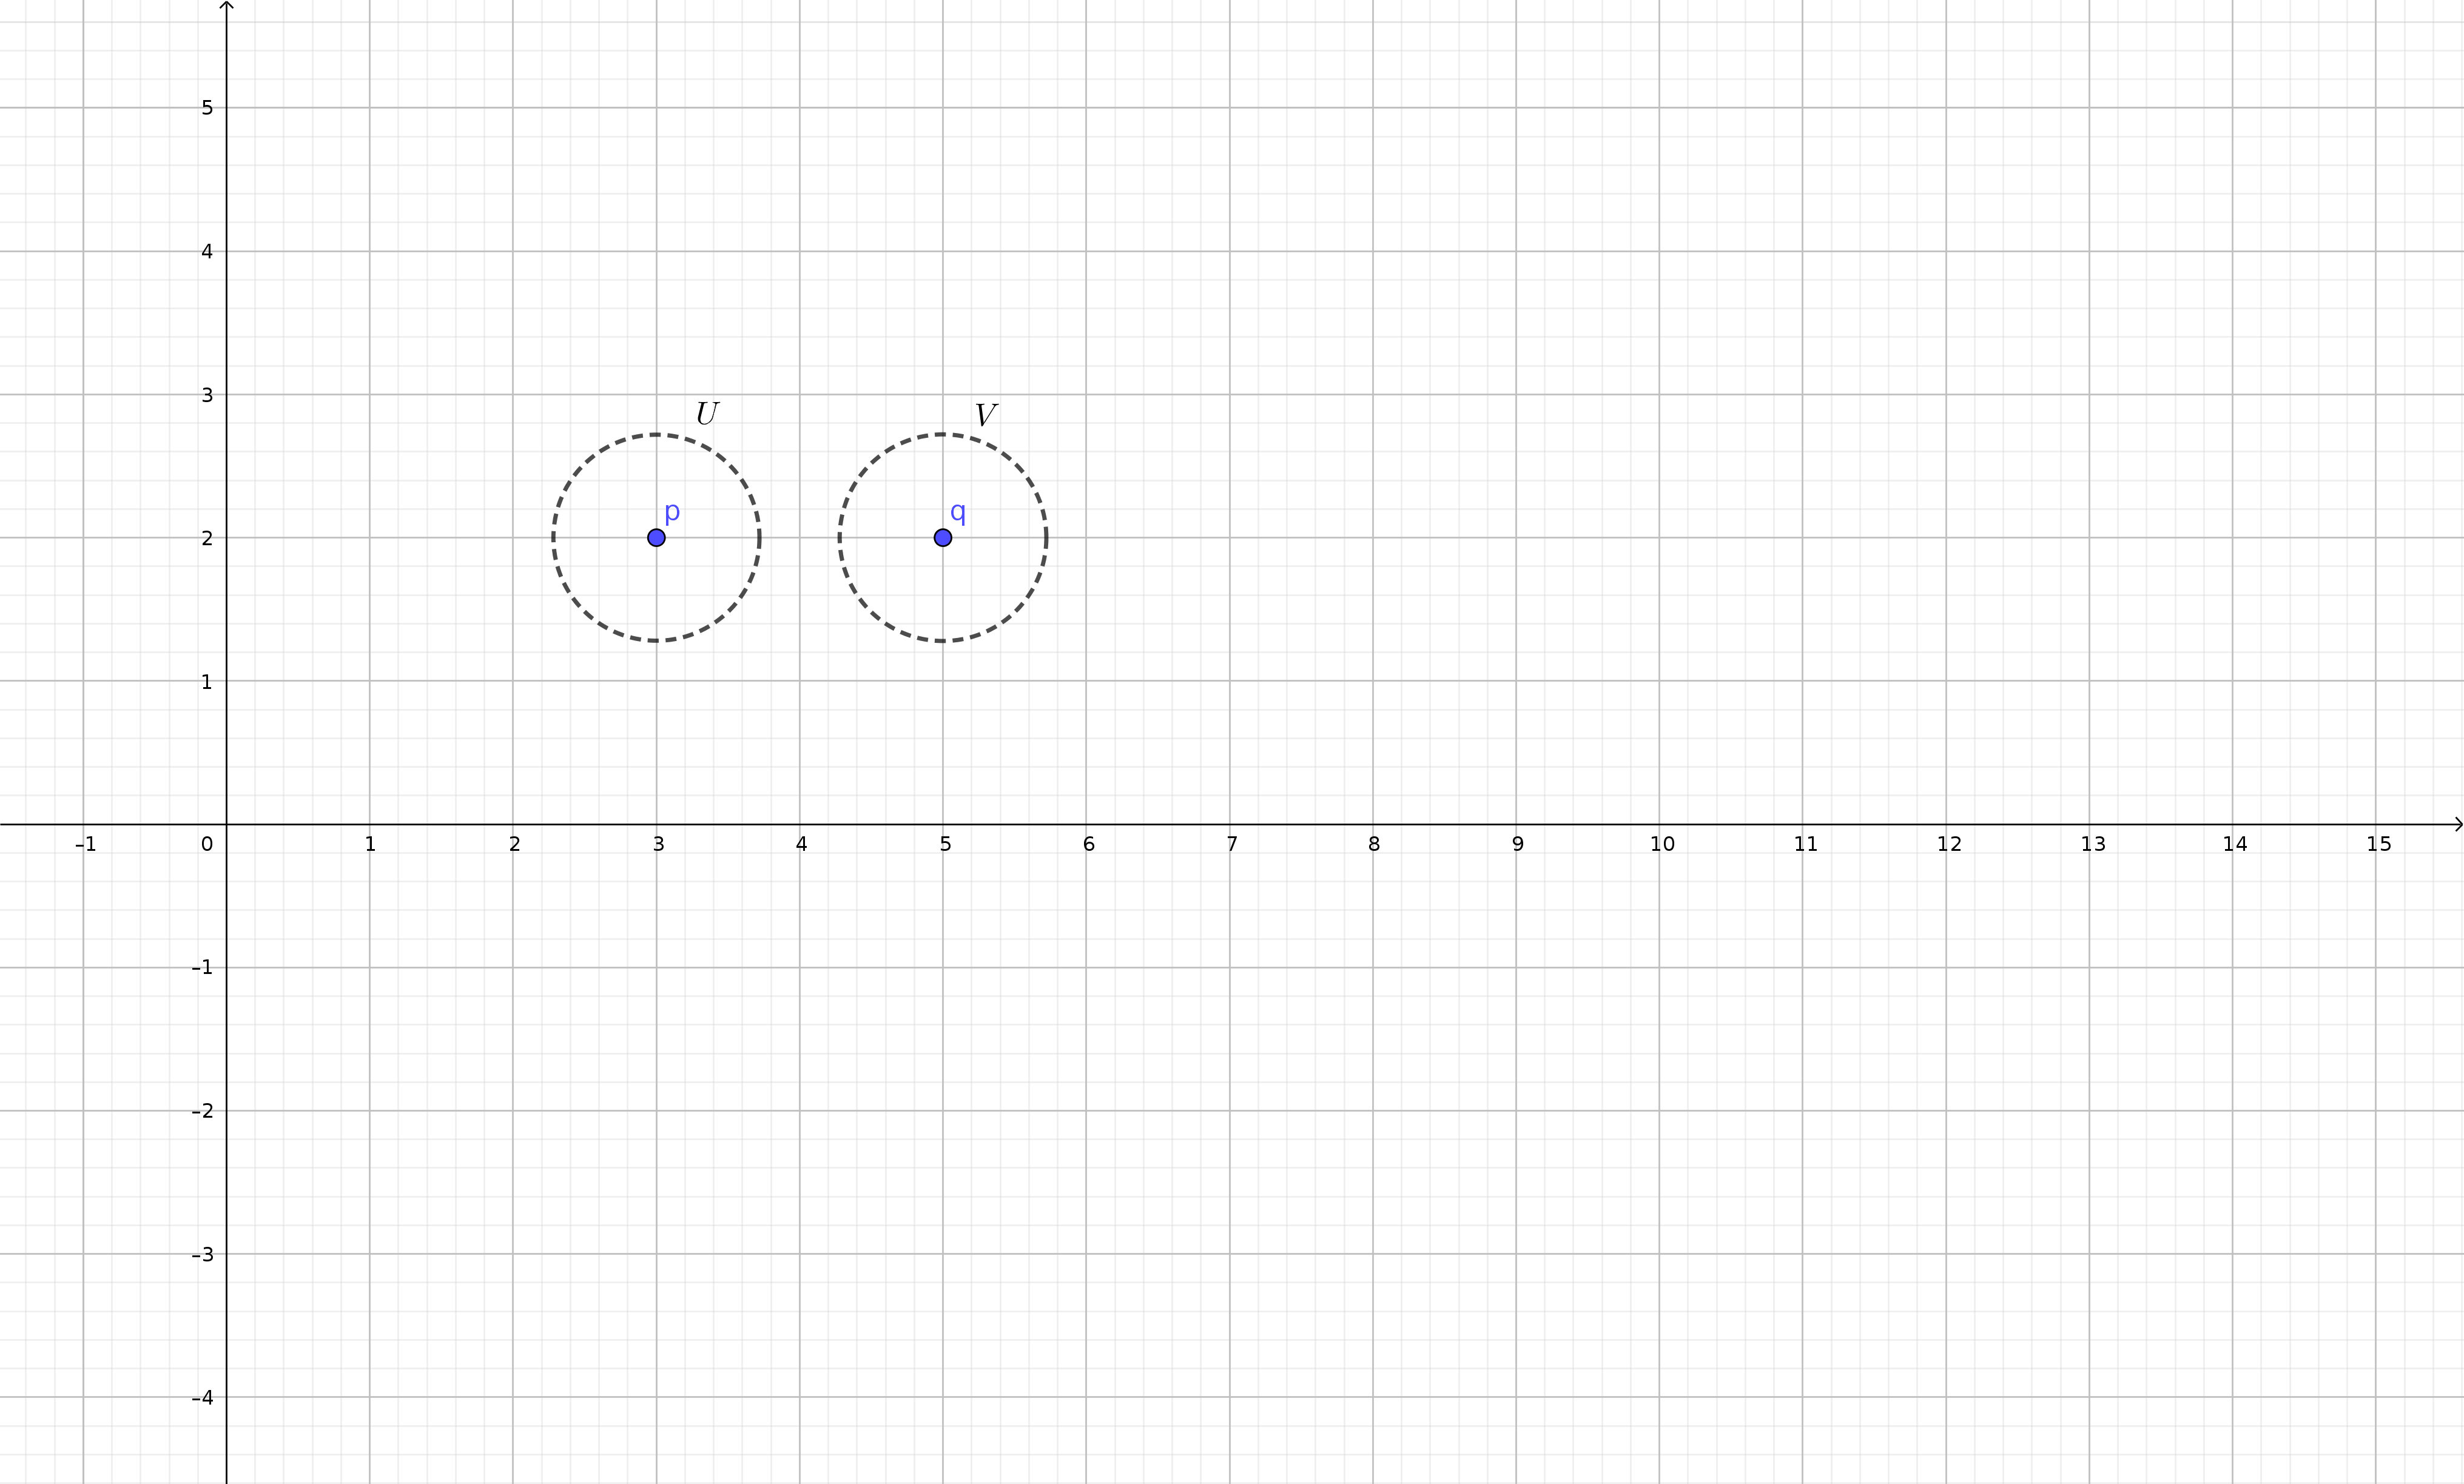
\includegraphics[trim = {3.8cm 5.8cm 9.7cm 2.8cm}, width=0.5\textwidth, clip]{Figures/metric-spaces-Hausdorff-spaces-v2.png}
		\caption{Visualization for why a metric space is a Hausdorff space.}
		\label{metric-space-Hausdorff-space}
	\end{figure} 
	A visualization is shown in Fig. \ref{metric-space-Hausdorff-space}. To prove this more rigorously, define $U := B_{r}(p)$ and $V:=B_{r}(q)$ with radius $r := \frac{d(p, q)}{2}$, where from Theorem \ref{open-balls-open} we know that $U$ and $V$ are open. Suppose $U\cap V = \emptyset$ would not hold. Then there exists a $z\in U\cap V$ with 
	\begin{align}
		d(p, z) < \frac{d(p, q)}{2}
	\end{align}
	and 
	\begin{align}
		d(q, z) < \frac{d(p, q)}{2}. 
	\end{align}
	Therefore, by the triangle inequality for metric spaces, we have: 
	\begin{align}
		d(p, q) \leq d(p, z) + d(q, z) < d(p, q), 
	\end{align}
	which is clearly a contradiction. 
\end{proof}

\begin{theorem}
	Let $X$ be a Hausdorff space, and $K\subset X$ compact, then $K$ is closed.
\end{theorem}

\begin{proof}[Proof \cite{topology-singh, 1329787}]
	Fix $x\in X\setminus K$, then for each $y\in K$, there exist open sets $U_y, V_y\subset X$ s.t. $x\in U_y$ and $y\in V_y$ with $U_y\cap V_y = \emptyset$, since $x\ne y$. Clearly, the family $\{V_{y}\mid y\in K\}$ of subsets of $X$ is an open covering of $K$, and since $K$ is compact, there exist finitely many points $y_1, \dots, y_n$ with $n\in\mathbb N$ and $y_k\in K$ for all $k\in \{1, \dots, n\}$ s.t. $K \subset \bigcup_{k=1}^{n}V_{y_k} =: V$. Define $U := \bigcap_{k=1}^{n}U_{y_k}$ and note that $x\in U$.
	
	We now show that $U \cap V \ne \emptyset$ via contradiction. Assume there is a $z\in U\cap V$, i.e. $z\in U$ and $z\in V$. This implies that $z\in U_{y_k}$ for all $k\in \{1, \dots, n\}$ and that there is a $k'\in\{1, \dots, n\}$ s.t. $z\in V_{y_{k'}}$. However, this is a contradiction to $U_{y_{k'}} \cap V_{y_{k'}} = \emptyset$. 
	
	Since $U\cap V\ne\emptyset$, $x\in U\subset X\setminus V\subset X\setminus K$, and since $x\in X\setminus K$ was arbitrary, by Theorem \ref{thrm:open_via_nbd}, $X\setminus K$ is open, implying that $K$ is closed.
\end{proof}

\begin{defn}
	Let $(X, \tau)$ be a topological space. Then it is said to be \textit{second countable} if $\tau$ has a countable basis. 
\end{defn}

\begin{exmp}
	For any $n > 0$, the topological spaces $\mathbb R^n$ are second countable. 
\end{exmp}

\begin{remark}
	Metric spaces are not automatically second countable. For example, take an uncountable set $X$, endow it with the discrete metric and because of Example \ref{exmp:basis_discrete_metric}, \ref{exmp:metric_topology},  the topological space $X$ is not second countable, since $X$ is uncountable. 
\end{remark}	

\subsection{Continuity and Homeomorphisms}

In topological spaces (which are not necessarily metrizable), we define continuity as follows \cite{topology-singh}:

\begin{defn}\label{defn:continuity_topological_spaces}
	Let $(X, \tau_X)$ and $(Y, \tau_Y)$ be topological spaces. Then a function $f: X \to Y$ is called continuous on $X$ if for every $U\in \tau_Y$, $f^{-1}(U) := \{ x\in X \mid f(x)\in U \} \in \tau_X$.
\end{defn}

\begin{exmp}
	Let $(X, \tau_X)$ be a topological space, then the identity $\text{id}: X\to X$ is continuous.
\end{exmp}

\begin{proof}
	Let $U\in \tau_X$, then $f^{-1}(U) = U\in\tau_X$.
\end{proof}

\begin{remark}
	In other words, the preimage of an open set is always open. For topological spaces that are metrizable, the $\epsilon$-$\delta$ definition of continuity as in Def. \ref{defn:continuity} is equivalent to the preceding definition, cf. Theorem \ref{thrm:preimages_continuous_functions}.
\end{remark}

\begin{theorem}\label{thrm:continuity_sub_basis}
	Let $(X, \tau_X)$ and $(Y, \tau_Y)$ be topological spaces, and $\mathscr B$ a basis or a subbasis for $\tau_Y$, then $f: X\to Y$ is continuous iff the inverse image under $f$ of every member of $\mathscr B$ is open in $\tau_X$ \cite{topology-singh}. 
\end{theorem}

\begin{proof}
	Let $\mathscr B$ be a basis, then if $f$ is continuous, $f^{-1}(B)\in\tau_X$ for all $B\in \mathscr B$. Conversely, every open set in $\tau_Y$ can be written as the union of basis members, i.e. $V = \bigcup_{i\in I}B_i$, where $I$ is an index set, and by Theorem \ref{thrm:set_theory_unions_intersects_preimages}, $$f^{-1}(V) = f^{-1}\left(\bigcup_{i\in I}B_i\right) = \bigcup_{i\in I}f^{-1}(B_i)\in \tau_X,$$ since $f^{-1}(B_i)\in\tau_X$ for all $B_i\in\mathscr B$.
	
	If $\mathscr B$ is a subbasis for $\tau_Y$, and $f$ is continuous, then $f^{-1}(B)\in \tau_X$ for all $B\in\mathscr B$, since $\mathscr B\subset \tau_Y$. Conversely, let $f^{-1}(B) \in \tau_X$ for all $B\in\mathscr B$. We know that each $V\in \tau_Y$ can be written as the union of a finite intersection of members of $\mathscr B$, i.e. $V = \bigcup_{i\in I}\left(\bigcap_{j\in J}B_{i, j}\right)$, where $J$ is a finite index set and $I$ an index set, and by Theorem \ref{thrm:set_theory_unions_intersects_preimages},
	$$f^{-1}(V) = f^{-1}\left(\bigcup_{i\in I}\left(\bigcap_{j\in J}B_{i, j}\right)\right) = \bigcup_{i\in I}\left(\bigcap_{j\in J}f^{-1}(B_{i, j})\right)\in \tau_X,$$
	since $f^{-1}(B_{i, j})\in \tau_X$ for all $B_{i, j}\in \mathscr B$.
\end{proof}

\begin{exmp}
	Consider the function $f: [0, 2\pi)\to \mathbb S^1, t\mapsto e^{it}$, where $$\mathbb S^1 := \left\{e^{it} \mid t\in [0, 2\pi)\right\} = \left\{(x, y)\in\mathbb R^2 \mid x^2 + y^2  = 1\right\}$$ is the unit circle in $\mathbb R^2$. Let $[0, 2\pi)$ be equipped with the order topology, cf. Definition \ref{defn:order_topology}, and $\mathbb S^1\subset\mathbb R^2$ be equipped with the subspace topology, cf. Theorem \ref{thrm:subspace_topology}, where $\mathbb R^2$ is equipped with the Euclidean topology.
\end{exmp}

\begin{proof}
	By Theorem \ref{thrm:subspace_basis}, the collection of all open arcs of $\mathbb S^1$ is a basis for the subspace topology on $\mathbb S^1$, since any open arc is the intersection of the full circle with an open ball. Figure \ref{fig:open_arc} visualizes this.
	\begin{figure}[h]
		\centering
		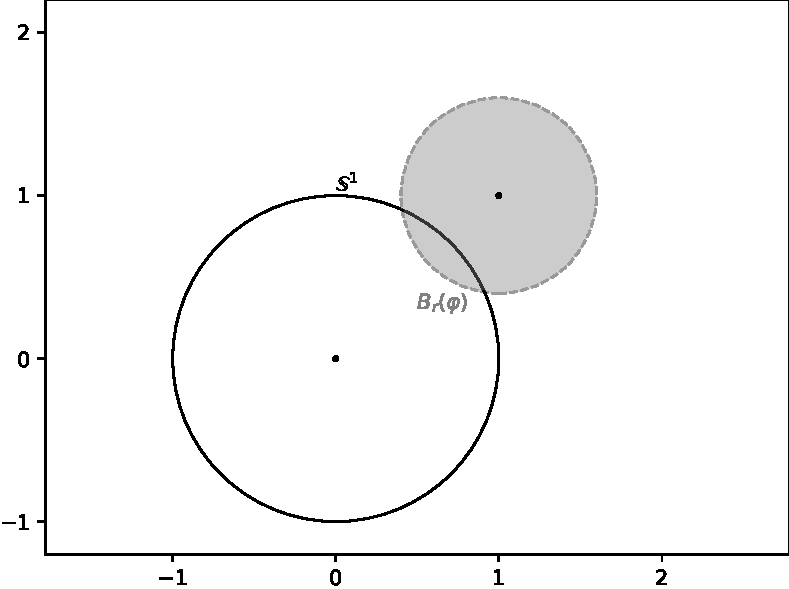
\includegraphics[width=0.6\textwidth]{Figures/circles_intersection_arc.pdf}
		\caption{Every open arc is the intersection of $\mathbb S^1$ with an open ball.}
		\label{fig:open_arc}
	\end{figure}
	
	Let $G\subset \mathbb S^1$ be an open arc that does not contain $1\in \mathbb S^1$, then $f^{-1}(G) = (a, b)$, where $0 < a < b < 2\pi$. 
	
	If $G$ does contain $1\in\mathbb S^1$, then $f^{-1}(G) = [0, a) \cup (b, 2\pi)$, where $0 < a < b < 2\pi$. Thus, regardless of whether $G$ contains $1$, $f^{-1}(G)$ is open in $[0, 2\pi)$ -- note that $f^{-1}(G)$ is open in $\mathbb R$ -- and thus $f$ is continuous by Theorem \ref{thrm:continuity_sub_basis}.
\end{proof}

\begin{theorem}\label{thrm:composition_continuous_functions}
	Let $(X, \tau_X)$, $(Y, \tau_Y)$ and $(Z, \tau_Z)$ be topological spaces, and $f: X\to Y$, $g: Y\to Z$ be continuous, then $g\circ f: X\to Z$ is continuous as well.
\end{theorem}

\begin{proof}
	Let $W\in\tau_Z$, then $(g\circ f)^{-1}(W) = (f^{-1}\circ g^{-1})(W)$, and since $g^{-1}(W)\in \tau_Y$, this implies that $(f^{-1}\circ g^{-1})(W)\in\tau_X$.
\end{proof}

\begin{theorem}\label{thrm:image_of_cont_func_on_comp_top_space_is_compact}
	Let $X$ be a compact topological space, $Y$ a topological space and $f: X\to Y$ a continuous function, then $f(X)$ is a compact subspace of $Y$.
\end{theorem}

\begin{proof}[Proof \cite{226328}]
	Let $\{U_i\}_{i\in I}$ be an open cover of $f(X)$. Since $f$ is continuous, $f^{-1}(U_i)$ is open in $X$ for every $i\in I$. Note that $\{f^{-1}(U_i)\}_{i\in I}$ is an open cover of $X$, since  $$f(X)\subset \bigcup_{i\in I}U_i\Rightarrow X\subset f^{-1}(f(X))\subset f^{-1}\left(\bigcup_{i\in I}U_i\right) = \bigcup_{i\in I}f^{-1}(U_i),$$ cf. Eq. \eqref{eq:preimage_image_of_set}. Since $X$ is compact, there is a finite subcover $\left\{f^{-1}(U_j)\right\}_{j\in J}$ of $X$, where $J\subset I$ is finite. Thus,
	$$X = \bigcup_{j\in J}f^{-1}(U_j)\Rightarrow f(X) = f\left(\bigcup_{j\in J}f^{-1}(U_j)\right) = \bigcup_{j\in J}f(f^{-1}(U_j))\subset \bigcup_{j\in J}U_j,$$
	cf. Eq. \eqref{eq:image_preimage_of_set}, which shows that every open cover of $f(X)$ has a finite subcover.
\end{proof}

\begin{defn}[Homeomorphism \cite{topology-singh}] A \textit{homeomorphism} between two topological spaces $X$ and $Y$ is an invertible function $f: X\rightarrow Y$ such that $f$ and $f^{-1}$ are continuous. 
\end{defn}

\begin{exmp}
	The Euclidean space $\mathbb R^n$, equipped with the usual topology, is homeomorphic to the open ball $B_{r}(\varphi) =  \{x\in\mathbb R^n \mid \lvert\lvert x-\varphi \rvert\rvert < r \} \subset \mathbb R^n$ (consider the open ball as a metric space with the \textit{induced metric} from the whole space of $\mathbb R^n$ and then equip it with the usual topology on a metric space given by the open sets). 
\end{exmp}

\begin{proof}
	Consider the map $$f: \mathbb R^n\rightarrow B_r(\varphi), \ x\mapsto \frac{r\cdot (x-\varphi)}{1+\lvert\lvert x-\varphi\rvert\rvert}.$$ Obviously, $f$ is continuous with inverse $$f^{-1}: B_r(\varphi)\rightarrow \mathbb R^n, \ x \mapsto \frac{x}{r-\lvert\lvert x\rvert\rvert}+\varphi,$$ which is also continuous. One can easily show that $f$ and $f^{-1}$ are inverses to each other. Thus, $f$ describes a homeomorphism. 	
\end{proof}

\begin{exmp}[Stereographic projection]
	The unit sphere $S^n$, embedded in $\mathbb R^{n+1}$, without the north pole, i.e. $S^n\backslash \{p\} \subset \mathbb R^{n+1}$, where $S^n := \{ x\in\mathbb R^{n+1} \mid \norm{x}{2} = 1 \}$ and $p := \{ x\in\mathbb R^{n+1} \mid x_i = 0 \ \forall i\in[1, n], x_{n+1} = 1 \}$, is homeomorphic to $\mathbb R^n$ (consider the unit sphere as a metric space with the \textit{induced metric} from the whole space of $\mathbb R^{n+1}$ and then equip it with the usual topology on a metric space given by the open sets). 
\end{exmp}
\begin{proof}
	Consider the map 
	\begin{align}
		f: S^n\backslash\{p\}\rightarrow \mathbb R^n, \ x\mapsto \frac{1}{1-x_{n+1}}\begin{pmatrix} x_1, \dots, x_n \end{pmatrix}^T. 
	\end{align}
	Obviously, $f$ is continuous. Its inverse is given by 
	\begin{align}\label{stereographic_map_inverse}
		f^{-1}: \mathbb R^n \rightarrow S^n\backslash\{p\}, \ x\mapsto \begin{pmatrix} 2x_1/ \left(1+\norm{x}{2}^2\right)\\ \vdots\\ 2x_n/\left(1+\norm{x}{2}^2\right) \\[4pt] 1-2/\left(1+\norm{x}{2}^2\right) \end{pmatrix}.  
	\end{align}
	It is trivial to show that $f$ and $f^{-1}$ are inverses to each other. One can also easily show that $\norm{f^{-1}(x)}{2} = 1$; thus, $f^{-1}$ does indeed bring us to the unit ball $S^n$. 
	To see that $f^{-1}$ is continuous, note that all components are continuous and thus, according to Lemma \ref{continuity_vector_components}, the function itself is continuous. 
\end{proof} 

\begin{theorem}\label{thrm:composition_homeomorphisms}
	Let $(X, \tau_X)$, $(Y, \tau_Y)$ and $(Z, \tau_Z)$ be topological spaces, and $f: X\to Y$, $g: Y\to Z$ be homeomorphisms, then $g\circ f: X\to Z$ is a homeomorphism.
\end{theorem}

\begin{proof}
	The composition of bijective functions is bijective again. From Theorem \ref{thrm:composition_continuous_functions}, we know that $g\circ f$ is continuous. To show the continuity of $(g\circ f)^{-1}: Z\to X$, note that if $U\in\tau_X$, then $(g\circ f)(U) = g(f(U))$, and since $f$ and $g$ are homeomorphisms, we have $f(U)\in \tau_Y$, and thus $g(f(U))\in\tau_Z$.
\end{proof}

\begin{theorem}\label{thrm:identity_homeomorphism_topologies_coincide}
	Let $(X, \tau_1)$ and $(X, \tau_2)$ be topological spaces. The identity map $\iota: (X, \tau_1)\to (X, \tau_2), x\mapsto x$ is a homeomorphism iff $\tau_1 = \tau_2$.
\end{theorem}

\begin{proof}[Proof \cite{3164142}]
	Let $\iota: (X, \tau_1)\to (X, \tau_2), x\mapsto x$ be a homeomorphism. We know that $\tau_1$ is a base generating itself, as is $\tau_2$ a base generating itself. Consider $U\in \tau_2$, then for all $x\in U$, $x\in \iota^{-1}(U) = U\in \tau_1$, since $\iota$ is continuous. Also, for any $U\in \tau_1$ and $x\in U$, $x\in \iota(U) = U\in \tau_2$, since $\iota^{-1}$ is continuous. Thus, by Corollary \ref{corollary:equality_of_topologies}, $\tau_1 = \tau_2$.
	
	Conversely, let $\tau_1 = \tau_2$, and consider $\iota: (X, \tau_1)\to (X, \tau_2), x\mapsto x$. Let $U\in \tau_2$, then $\iota^{-1}(U) = U\in \tau_1 = \tau_2$, and thus $\iota$ is continuous. Let $U\in\tau_1$, then $\iota(U) = U\in \tau_2 = \tau_1$, and thus also $\iota^{-1}$ is continuous. Further, $\iota$ is bijective, implying that $\iota$ is a homeomorphism.
\end{proof}